
%%%%%%%%%%%%%%%%%%%%%%%%%%%%%%%%%%%%%%%%%
% The Legrand Orange Book
% LaTeX Template
% Version 2.0 (9/2/15)
%
% This template has been downloaded from:
% http://www.LaTeXTemplates.com
%
% Mathias Legrand (legrand.mathias@gmail.com) with modifications by:
% Vel (vel@latextemplates.com)
%
% License:
% CC BY-NC-SA 3.0 (http://creativecommons.org/licenses/by-nc-sa/3.0/)
%
% Compiling this template:
% This template uses biber for its bibliography and makeindex for its index.
% When you first open the template, compile it from the command line with the 
% commands below to make sure your LaTeX distribution is configured correctly:
%
% 1) pdflatex main
% 2) makeindex main.idx -s StyleInd.ist
% 3) biber main
% 4) pdflatex main x 2
%
% After this, when you wish to update the bibliography/index use the appropriate
% command above and make sure to compile with pdflatex several times 
% afterwards to propagate your changes to the document.
%
% This template also uses a number of packages which may need to be
% updated to the newest versions for the template to compile. It is strongly
% recommended you update your LaTeX distribution if you have any
% compilation errors.
%
% Important note:
% Chapter heading images should have a 2:1 width:height ratio,
% e.g. 920px width and 460px height.
%
%%%%%%%%%%%%%%%%%%%%%%%%%%%%%%%%%%%%%%%%%

%----------------------------------------------------------------------------------------
%	PACKAGES AND OTHER DOCUMENT CONFIGURATIONS
%----------------------------------------------------------------------------------------

\documentclass[12pt,fleqn]{book} % Default font size and left-justified equations

%----------------------------------------------------------------------------------------

\input{structure} % Insert the commands.tex file which contains the majority of the structure behind the template

%%agregué


\usepackage[hang, small,labelfont=bf,up,textfont=it,up]{caption} % Custom captions under/above floats in tables or figures
%\usepackage[left=1.5cm,top=2.5cm,right=1.5cm,bottom=2.5cm]{geometry}
\usepackage{booktabs} % Horizontal rules in tables
\usepackage{float} % Required for tables and figures in the multi-column environment - they




\usepackage{graphicx} % paquete que permite introducir imágenes

\usepackage{booktabs} % Horizontal rules in tables
\usepackage{float} % Required for tables and figures in the multi-column environment - they


\usepackage{color}
\usepackage{colortbl}
\usepackage{bm}


%%%%%%%%%%%%%%%%%%%%%%%%%%%%%%%%%propia
\usepackage[utf8]{inputenc}
%\usepackage[english]{babel}
\usepackage{textcomp}
 
\usepackage[nottoc]{tocbibind}

\numberwithin{equation}{section} % Number equations within sections (i.e. 1.1, 1.2, 2.1, 2.2 instead of 1, 2, 3, 4)
\numberwithin{figure}{section} % Number figures within sections (i.e. 1.1, 1.2, 2.1, 2.2 instead of 1, 2, 3, 4)
\numberwithin{table}{section} % Number tables within sections (i.e. 1.1, 1.2, 2.1, 2.2 instead of 1, 2, 3, 4)


\setlength\parindent{0pt} % Removes all indentation from paragraphs - comment this line for an assignment with lots of text

%%hasta aquí


\begin{document}

%----------------------------------------------------------------------------------------
%	TITLE PAGE
%----------------------------------------------------------------------------------------

\begingroup
\thispagestyle{empty}
\begin{tikzpicture}[remember picture,overlay]
\coordinate [below=9cm] (midpoint) at (current page.north);
\node at (current page.north west)
{\begin{tikzpicture}[remember picture,overlay]
\node[anchor=north west,inner sep=0pt] at (0,0)
{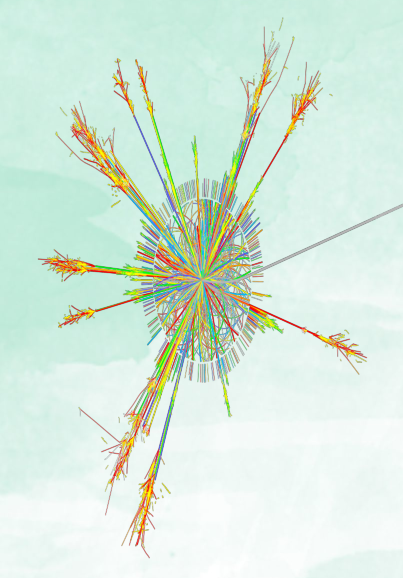
\includegraphics[width=\paperwidth]{portada}}; % Background image
\draw[anchor=north] (midpoint) node [fill=ocre!60!white,fill opacity=0.4,text opacity=1,inner sep=1cm]{\Huge\centering\bfseries\sffamily\parbox[c][][t]{\paperwidth}{\centering Evaluación de eficiencia de atenuación de elementos de protección para trabajadores expuestos en el área de radiología bajo la herramienta FrameWork-Geant4.\\[15pt] % Book title
%Evaluación de eficiencia de atenuación de radiación para trabajadores expuestos en el área de radiología bajo la técnica de Geant4
%\textit{Caso de uso:Chaleco plomado en servicio de radiología}\\[15pt] % Book title
{\Large  Isabel Alejandra Morales Salamanca}\\[20pt] % Subtitle
{\huge Universidad Distrital Francisco José de Caldas\\}}}; 
% Author name
\end{tikzpicture}};
\end{tikzpicture}
\vfill
\endgroup


%----------------------------------------------------------------------------------------
%	COPYRIGHT PAGE
%----------------------------------------------------------------------------------------

%\newpage
%~\vfill
%\thispagestyle{empty}

%\noindent Copyright \copyright\ 2013 John Smith\\ % Copyright notice

%\noindent \textsc{Published by Publisher}\\ % Publisher

%\noindent \textsc{book-website.com}\\ % URL

%\noindent Licensed under the Creative Commons Attribution-NonCommercial 3.0 Unported License (the ``License''). You may not use this file except in compliance with the License. You may obtain a copy of the License at \url{http://creativecommons.org/licenses/by-nc/3.0}. Unless required by applicable law or agreed to in writing, software distributed under the License is distributed on an \textsc{``as is'' basis, without warranties or conditions of any kind}, either express or implied. See the License for the specific language governing permissions and limitations under the License.\\ % License information

%\noindent \textit{First printing, March 2013} % Printing/edition date

%----------------------------------------------------------------------------------------
%	TABLE OF CONTENTS
%----------------------------------------------------------------------------------------

\chapterimage{intro} % Table of contents heading image

%\chapterimage{chapter_head_1.pdf} % Table of contents heading image

\pagestyle{empty} % No headers

 \tableofcontents % Print the table of contents itself

\cleardoublepage % Forces the first chapter to start on an odd page so it's on the right

\pagestyle{fancy} % Print headers again

%----------------------------------------------------------------------------------------
%	PART
%----------------------------------------------------------------------------------------

\part{Parte Uno}

%----------------------------------------------------------------------------------------
%	CHAPTER 1
%----------------------------------------------------------------------------------------
\chapterimage{ima2*} % Chapter heading image

\chapter{Introducción}
%\section{Introducción}\index{Modelo Logit}

La radiación ha estado presente desde los inicios del universo. Desde su aparición sobre la tierra y posteriormente la compresión de su naturaleza, ha aportado a la humanidad incontables beneficios, enmarcando sus usos y aplicaciones en un dualidad, tanto para fines beneficios como destructivos.
En efecto, aun prevalecen en la memoria los efectos nefastos de la radiación en los seres humanos afectados por los desastres de Hiroshima, Chernobil, y Fukushima, y ello ha permitido que permanezca un sentimiento negativo de desconfianza y temor hacia la radiación.



Pese a ello, el control de la energía de las radiaciones ha permitido el progreso en diversas disciplinas del saber, en especial en la medicina, abriendo nuevas posibilidades en el diagnostico, tratamiento (terapias) y prevención de enfermedades cancerígenas. Además de sus cuantiosos beneficios y usos, en la medicina, la radiación también se ha impregnado en otra áreas de aplicación  como en la academia, en la tecnología y la industria. Aplicaciones en esta dirección son las que motivan el estudio de este trabajo, ya que permiten evaluar una amplia gama de usos en diferentes áreas de empleo.


La aplicaciones mencionadas tienen como eje fundamental al fenómeno de la radiación.Se comprende a la radiacion, como la propagacion de enrgia en forma de ondas electromagnéticas o particulas subatomicas atraves del espacio vacion a de un medio material.CONTINUAR TRADUCTOR


EXTENDER CUAL ES EL OBJETIVO DE LA RADIACIÓN bajo la base de protección radiológica(radiacion-protección y atenuacion)

%Estas características han sido explotadas en áreas tales como la medicina,la agricultura y la ingeniería. En la medicina (área de interés en este estudio) por ejemplo bajo la técnica de  radioterapia, las propiedades de la radiación buscan disminuir la proliferación de las células malignas(cancerígenas).En esta y en otras técnicas empleadas en el área, es necesario hacer uso de detectores que permitan monitorear la radiación a la que los trabajadores,pacientes y publico se encuentran potencialmente expuestos. 


5.
En la actualidad, monitorear la radiación, es un campo en el cual, la simulación por ordenador es una herramienta dinamica de implementar,accesible y económica.En general, la simulación ha permeado la ciencia debido a:  


SIMULACION IMPORTANCIA,SIMULACION EN AREAS COMO LA MEDICINA

Haciendo uso del lenguage C++ y usando el software GEANT4,herramienta desarrollada  por el CERN en la ultima decada,se realiza una simulacion que permite constituir estructuras  geometricas donde se logra producir procesos fisicos medibles del proceso especifico que se da de manera material y en tiempo real dentro de un escenario medico. 
La simulacion apartir de uso del software,se ha convertido en una herramienta eficaz para verificar tratamientos en el area de la medicina (radioterapia con aceleradores),de igual forma es usado para modelar aquellos componentes propios de los detectores usados en dosimetria clinica y para imitar las interacciones de la radiacion en el paciente.




La estructura de este documento y el manejo  de los temas están establecidos de la siguiente manera: En el primer capitulo se establece la fundamentación teórica. Allí se desarrolla los conceptos básicos de las interacciones electromagnéticas de las partículas con la materia.

 En el segundo capitulo, se detalla los lineamientos físicos asociados a a las librerías empleadas para el laboratorio virtual. Básicamente en este capitulo se retoman los conceptos descritos en el  primer capitulo para establecerlos como la base de funcionamiento del experimento a simular. En el tercer capitulo se detalla la metodología de construcción del modelo a simular. Este capitulo también incluye el procesamiento de la información obtenida a través del laboratorio virtual.El ultimo capitulo se centra en los resultados, los análisis, las conclusiones y perspectivas para futuros trabajos encaminados en el mismo sentido.










\section{Objetivo General}\index{Objetivo General}
Estudiar la atenuación presente en una estructura plomado como elemento de protección radiológica en la practica de radiología, mediante configuraciones relacionadas con los parámetros de espesor y energía.


%(\textit{Chaleco})
\section{Objetivos Específicos}
\index{Objetivos Específicos}
\begin{itemize}

\item Simular el fenómeno físico, en el que la fuente son haces mono energéticos dirigidos a un blanco (chaleco plomado).   
%Explorar la teoría correspondiente a la física relacionada con la interacción radiación materia y su aplicación desde la herramienta computacional Geant4

\item Corroborar que el porcentaje de atenuación obtenida mediante el laboratorio experimental y el laboratorio simulado,se encuentran dentro del rango del porcentaje de atenuación establecido por  el proveedor del chaleco.   
%Obtener resultados experimentales a partir del montaje simulado del conjunto fuente-elemento atenuador.

\item Comparar los resultados teóricos y experimentales de la atenuación presente en el uso del chaleco como elemento de protección radiológica. 
\item Encontrar la tasa de atenuación para un chaleco con diferentes configuraciones(espesor-energía).

\end{itemize}
%----------------------------------------------------------------------------------------
%	CHAPTER 2
%----------------------------------------------------------------------------------------

\chapterimage{ima30*}
\chapter{Interacción de fotones con materia}

%\section{Modelo Logit}\index{Modelo Logit}

%\subsection{Introducción}\index{Introducción}
\textbf{Introducción}\index{Introducción}
\\\\
El siguiente capítulo proporciona una introducción a la física moderna y cubre elementos básicos sobre radiación y  teoría electromagnética. Los primeros descubrimientos y explicación de las mismas se dan inicialmente con 
Heinrich Hertz en 1887 donde establece que la radiación electromagnética al incidir sobre una  superficie metálica esta puede expulsar partículas cargadas,luego vino Thompson Joseph quién probó  a partir de un tubo que los rayos catódicos presentes tenían naturaleza de corpúsculo,partículas a las que luego llamo electrones, posteriormente Bohr y Rutherford desarrollaron experimentos que guiaron la comprensión de la estructura del átomo.
\\\\
Tomando a los fotones como un cuanto de radiación electromagnética, gracias a la explicación de Einstein donde propone que dicha radiación era cuantificada de forma semejante a aquellos niveles propuestos por Plank en el año 1900. Los elementos mencionados anteriormente  forman el conjunto importante de conocimiento para estudiar la física inmersa en la medicina bajo los efectos de la radiación.
\\\\

%desderevision

\section{Radiación}
La radiación como concepto fundamental,base para nuestro estudio se define como aquella energía capaz de transportarse  a través de la materia o el espacio,ya sea en forma de onda o partícula como ya fue antes demostrado bajo la teoría dual, característica de la luz.Su obtención se puede dar de dos formas distintas:bajo el proceso de interacción de una partícula con la materia o gracias a la desintegración radiactiva de un radionúclido (un átomo inestable), donde la radiación emitida de este proceso depende de las características propias del radionúclido específicamente usado, mientras que aquella  emisión de radiación proveniente de  interacción, depende de la partícula que entra  del material con el que choca,y es teóricamente hablando posible predecir resultados estadísticos bajo esta técnica siempre y cuando se conozca suficiente interacción no solo de proceder de una partícula entrante en el proceso,sino de cantidades considerablemente grandes.  

Este proceso de la radiación puede describirse bajo dos características:su energía y tipo,tipos que se encuentran divididos en dos características fundamentales: partículas y electromagnéticas,la primera,radica en partículas que poseen energía y masa pero que a su vez pueden contar o no con carga eléctrica.Dentro del tipo de radiación en partículas se consideran aquellas tales como: los protones,neutrones, partículas alfa y beta, y la radiación electromagnética es aquella que radica en fotones\textquotedblleft paquete de luz\textquotedblright,partículas sin masa ni carga pero que si contienen energía electromagnética,una cantidad discreta de esta como lo detalla la teoría cuántica y dentro de este concepto se especifica que la luz ultravioleta,los rayos x,gamma y la luz visible también son fotones.


%libro
%La unidad de energía más común utilizada para describir la radiación es el electronvoltio (eV). Un electronvoltio es la cantidad de energía cinética que gana un electrón cuando se acelera a través de una diferencia de potencial de un voltio. La conversión a unidades SI es 1 eV = 1.6x10-19 julios. UneV es una unidad de energía muy pequeña, por lo que en muchas aplicaciones, es más común usar kiloelectronvoltios (1 keV = 1000 eV) o megaelectrvoltios (1 MeV = 1,000,000 eV).La radiación puede ser ionizante o no ionizante, dependiendo de su energía y capacidad de penetrar la materia. La radiación no ionizante, como la luz visible, no es dañina. Solo la radiación ionizante se discute en este curso. La ionización se trata con más detalle en la página 11.
%findelibro
\section{La radiación y el átomo }
Es a partir de la estructura del átomo que es posible explicar el fenómeno que para esta ocasión es pertinente estudiar,la radiación,puesto que la materia esta compuesta de ellos,quienes que encuentran formados por un núcleo,donde se encuentran los neutrones que no cuentan con carga eléctrica y los protones quienes tienen cargas positiva.

Cada uno de los átomos poseen un electrón en orbita para cada protón en el núcleo,permitiendo que el tomo quede eléctricamente neutro.A partir de esta característica es posible evidenciar que tipo de elemento se trata. Sin olvidar claro esta,su estructura atómica.Donde hay un \textquotedblleft X \textquotedblright  que denota el símbolo químico de un elemento en particular,un \textquotedblleft Z \textquotedblright que indica el numero atómico \textquotedblleft número de protones en el núcleo \textquotedblright quien revela la identidad química del elemento.Un \textquotedblleft A \textquotedblright numero másico,definido como la suma de la cantidad de protones y neutrones que se encuentran en el núcleo.Por ultimo un \textquotedblleft A-Z \textquotedblright que establece el numero de neutrones,es por esta razón que es posible encontrar elementos con diferente cantidad de neutrones y a la vez ser químicamente igual.Gracias a esta distribución y caracterización,se establece que cada disposición individual de neutrones y protones da lo que se conoce como un nucleido,y quienes contienen el mismo numero de protones se denominan isótopos,como aquellos isótopos del hidrógeno,el Deuterio y el Tritio que a su vez es un nucleido radiactivo o inestable.

%libro

%La estabilidad del núcleo está relacionada con su relación de neutrones a protones. Para elementos de bajo número atómico, se necesitan números aproximadamente iguales de neutrones y protones en el núcleo para la estabilidad. Para elementos de mayor número atómico, la relación aumenta a aproximadamente 1.6 a 1. A medida que un nucleido se aleja de esta relación estable, se producen cambios en el núcleo que tienden a llevar el producto a una disposición más estable. Este enfoque de la estabilidad se logra con uno o más de cinco (5) "modos de desintegración radiactiva".
%findelibro

%desderevision

\section{Decaimiento radiactivo}
--------------------------


El fenómeno de la radiactividad es el proceso de aquella desintegración espontánea de aquellos núcleos inestables que logran descomponerse en alguna otra combinación de nucleones con una menor masa.

Este proceso es un proceso estadístico,donde se tiene una   muestra determinada de  material radiactivo, al cual se le mide las desintegraciones por unidad de tiempo,lo que se denomina como actividad. 

\begin{equation}
 Actividad = -\frac{dN}{dt}
\end{equation}

Donde  N determina los átomos inestables del material.

De tal forma que aquel nucleido radiactivo se desintegra de manera espontánea a una velocidad dependiente del número de átomos originales presentes y de su constante de descomposición, lambda ($\lambda$),esta constante se define como la fracción instantánea de átomos que se descomponen por unidad de tiempo.
Cada nucleido radiactivo tiene su propia constante de descomposición especifica.
La tasa de cambio de tiempo instantáneo del número de átomos, N, para un radionúclido se establece como:

\begin{equation}
\frac{dN}{N}=-\lambda dt
\end{equation}
\begin{equation}
\int_{N_{0}}^{N_{t}}\frac{dN}{N}=\int_{0}^{t}\lambda dt
\end{equation}
\begin{equation}
ln\left [  \frac{N_{t}}{N_{0}}\right ]=-\lambda t
\end{equation}
\begin{equation}
\frac{N_{t}}{N_{0}}=e^{-\lambda t}
\end{equation}
\begin{equation}
N_{t}=N_{o}e^{-\lambda t}
\end{equation}

A principios del siglo XX se observaron aquellos tipos de decaimientos conocidos como $\alpha$, $\beta$ y $\gamma$,los mas comunes para entonces, procesos y fenómenos que se generaban a partir de la descomposición del núcleo y dónde a partir de aquella acción como principio se preservan  las leyes de conservación de energía, de masa, de momento lineal, de momento angular, de carga eléctrica y por ultimo la conservación de nucleones que determina  que el numero total de nucleones (\textbf{A}, el numero de masa) debe conservarse en una reacción nuclear de baja energía (aproximadamente menos de 938 MeV) o en la descomposición.Estos neutrones pueden convertirse en protones, y viceversa, pero el numero total de nucleones debe permanecer constante.

NO ENTENDI LA PAG 453

\subsection{Decaimiento alfa}

Generalmente el núcleo es particularmente estable con una energía de unión de $28,3$ MeV.Si los últimos dos protones y dos neutrones en un núcleo están unidos por menos de 28.3 MeV, se produce la emisión de una partícula alfa.

Esta desintegración alfa es posible, porque Q (energía liberada) es mayor a cero,de hecho, muchos de los núcleos por encima de  A=150, son aptos para una desintegración alfa.Aquellos núcleos pesados tienen una repulsión de Coulomb cada vez mas fuerte a medida que se adicionan protones. La expulsión de dos protones (junto con dos neutrones)  en forma de una partícula  $\alpha$  puede disminuir la energía de Coulomb y hacer que el núcleo resultante sea mas estable.

Para que ocurra esta desintegración , dos neutrones y dos protones se agrupan dentro del núcleo antes de la desintegración, en segundo lugar, la partícula alfa, incluso cuando ya se ha formado, tiene una gran dificultad para superar la atracción nuclear de los nucleones restantes para escapar.

GRAFICA DE LA PAG 454

Las energias cineticas de las particulas alfa emitidas desde los nucleos varían de 4 a 10 MeV. Es clasicamente imposible que las particulas alfa escapen, puesto que  la barrera de energia potencial es mayor que la energia cinetica,
EXPLICAR ESTO
Si proyectamos particulas de 5 MeV en un nucleo pesado, encontramos que la partícula alfa es repelida por la fuerza de Coulomb
..
y no logra acercarse lo suficiente como para sentir la atracción de la fuerza nuclear de corto alcance.Por esto es imposible que la partícula alfa alcance el núcleo. 


Pero entonces como explicar que la particula alfa pueda superar la barrera si se encuentra atrapada dentro de la barrera de potencial. Estas  particulas alfa pueden hacer un tunel a traves de la barrera, donde existe una pequeña  posibilidad de que la particula alfa aparezca en el otro lado de la barrera, posibilidad que depende de la altura y el ancho de la barrera.

El mayor porcentaje de probabilidad de tunelizacion corresponde a una vida util mas corta para el nucleido radiactivo

........
ESTO ERA LO DE ANTES DEL DOC PARA ANEXAR
En este tipo de decaimiento o desintegración, los nucleidos pesados no tienen una configuración estable de neutrones y protones,donde se obtiene la emisión de una partícula alfa que se compone de 2 protones y 2 neutrones,este proceso de desintegración se produce en aquellos nucleidos que tienen  un número atómico mayor a 82.Para lograr un decaimiento de este tipo se necesita una serie de desintegraciones alfa (así como beta) hasta lograr alcanzar un elemento estable más ligero. A diferencia de las partículas beta, estas partículas alfa se emiten con una energía discreta.
........

\subsection{Decaimiento Beta}
En este tipo de decaimiento los núcleos inestables pueden acercarse más a la línea de estabilidad, ya que los electrones no pueden existir dentro del núcleo,y en las  desintegraciones $\beta$ dicha particula $\beta$ se crea en el momento de la desintegración. 

Esta desintegración  $\beta$ es el reflejo de un tipo especial de fuerza, llamada simplemente la interacción débil. Los neutrinos se crean (o absorben) en procesos débiles, incluida la esta descomposición.

En el decaimiento $\beta ^{+}$ se produce un electron positivo, llamado positron$e^{+}$. El positron es la antiparticula del electron. En la desintegracion beta
el electron y el positron  se denominan normalmente $\beta ^{-}$ y $\beta ^{+}$, respectivamente, lo que facilita el recordar que el electron y el positron se crean en el ucleo durante la desintegracion beta

NO ENTENDI ESTO PAG12
Debido a que los electrones K-shell y L-shell 
---------------

\subsection{Decaimiento Beta menos}
Este tipo de decaimiento se da cuando la relación de neutrones con respecto a los protones es muy alta,por esta razón un neutrón se \textquotedblleft convierte \textquotedblright en un protón y un electrón que es expulsado del núcleo.Es este electrón al que se designa como \textquotedblleft partícula beta menos\textquotedblright o beta,partículas no se emiten con una única energía,sino con un espectro amplio de energías,debido a la división de la energía total de la desintegración entre la partícula beta y un neutrino, partícula que se emite al mismo tiempo que la partícula beta,quien contiene una masa considerablemente reducida y sin carga,quien transporta la energía liberada en cantidades distintas.Cada una de estas características le permiten viajar distancias extensas,perdiendo poca energía al penetrar materiales cercanos sin causar daños de tipo biológico.



%libroLa energía de la partícula beta expulsada es característica de cada nucleido y es un criterio utilizado para fines de identificación. En general, la energía de partículas promedio es aproximadamente 1/3 de la energía máxima posible
%flibro
\subsection{Decaimiento beta mas}
Se produce cuando la correspondencia entre neutrones con respecto a protones es baja,donde un proton se transforma en un neutrón y en una partícula beta mas \textquotedblleft un positrón\textquotedblright quien tiene na carga positiva,la misma masa de un electron y el cual es expulsado del átomo.

Su comportamiento es fielmente igual al del electron,con la diferencia de que cuando el positrón tiene contacto con un electrón libre, estas dos partículas al combinarse se aniquilan,proceso que da lugar a dos fotones con una energía (0.511 MeV / fotón).



\subsection{Captura de electrones}
Para que se logre este tipo de desintegración se forma un neutrón,gracias a que  uno de los electrones que orbitan es capturado por el núcleo y se combina con un protón.Este proceso disputa con la desintegración de positrones cuando hay una baja relación de neutrones a protones puesto que si el átomo no logra cumplir con la energía que requiere para que se de la descomposición de positrones, el proceso de desintegración se dará por captura de electrones, y cuando esto ocurre,existe una emisión de rayos X, los cuales son característicos del recién formado nucleido.

\subsection{Transición isomérica}
En este proceso cuando se da una emisión de una partícula y el núcleo del producto se encuentra en un estado meta-estable o en estado de excitación, y es aquí donde se emiten rayos gamma quienes se llevan el exceso de energía del núcleo parcialmente excitado luego de un evento de descomposición.Estos rayos gamma tienen una energía discreta.
 
\section{Vida Media}
Este concepto se refiere al tiempo que emplea y tardan la mitad de los atomos de una sutancia radiactiva en desintegrarse radiactivamente,o el tiempo que tarda la actividad de una muestra en reducirse a la mitad.


\title{El número de átomos restantes después de n semividas:}
\begin{equation}
 N=\frac{N_{0}}{2^{n}}
\end{equation}

$N_{0}=$ número inicial de átomos.
 
Asi que, para n=1, queda la mitad de los átomos iniciales; para n=2, quedan 1/4; para n=3, quedan 1/8, y así sucesivamente.


\subsection{Unidades de Radiactividad}
Puesto que es muy importante garantizar la equivalencia y uniformidad en las mediciones que se realicen es importante tener en cuenta la unidades de medida correspondientes a las variables a medir,y esta no es la excepción.

Cuando evidenciamos la siguientes expresión tenemos:
Número de átomos, N, que quedan en un instante particular en el tiempo
\begin{equation}
 A= \lambda  N
\end{equation}
\begin{itemize}
\item A = actividad,número instantáneo de átomos en descomposición por unidad de tiempo.
\end{itemize}


Actividad que se encuentra determinada de forma directa con la cantidad de material radiactivo en una muestra,actividad que se usa la unidad de curie (Ci).

\begin{itemize}

\item 1 curie = 3.7 x $10^{10}$ desintegraciones por segundo(dps)
\item 1 curie = 2.22 x $s10^{12}$ desintegraciones por minuto (dpm)

Sus unidades derivadas puesto que el curie es una cantidad muy grande,se establecen como:
\item 1 millicurie = (mCi) = 2.22 x $10^{9}$ dpm = $10^{-3}$ curies
\item 1 microcurie = ($\mu$ Ci) = 2.22 x $10^{6}$ dpm = $10^{-6}$ curies
\item 1 nanocurie = (nCi) = 2.22 x $10^{3}$ dpm = $10^{-9}$ curies
\item 1 picocurie = (pCi) = 2.22 dpm = $10^{-12}$ curies
\end{itemize}

Teniendo en cuenta que el material radiactivo se mide en unidades de actividad, la ecuación de descomposición se establece como:

\begin{equation}
A = A_{0}  e^{-\lambda t} 
\end{equation}

\begin{itemize}
\item A = Actividad después de un tiempo t
\item $A_{0}$ = actividad original de la muestra
\item $\lambda$= Constante de desintegración radiactiva igual a $\frac{0.693}{T_{\frac{1}{2}}}$
\item t = tiempo de decaimiento
  \end{itemize}

Ya que el Sistema Internacional (SI) de unidades ha definido el becquerel (Bq) como la unidad de actividad, igual a 1 desintegración por segundo.Tenemos:

1 Ci = 3.7 x $10^{10}$ Bq.

La actividad específica habitualmente se expresa en términos de la tasa de desintegración (dps o dpm), tasa de conteo (conteos / min, cpm, o conteos / seg, cps), o curies (o mCi, $\mu$ Ci) del radionúclido específico por unidad masa del elemento.Donde se tiene:

\begin{equation}
 SA=\lambda N
 \end{equation}
\begin{equation}
\lambda N = \lambda \frac{6.02 x 10^{23}}{m} Bq/g  
 \end{equation}

 
 \begin{itemize}
\item  SA = actividad especifica
\item  $\lambda$  = constante de decaimiento
\item N = número de átomos
\item m = masa molecular (gramos / mol).
\end{itemize}


\section{Interacción Radiación-Materia}

Aquella radiación que interactúa con la materia tiene la capacidad de ser absorbida o dispersada,el concepto de absorción en este contexto es importante e interesante puesto que:
\begin{itemize}
 \item Si los tejidos del cuerpo humano logran absorber dicha radiación,esta misma acción puede provocar lesiones biológicas
 \item Esta proceso de absorción es el fundamento sobre el cual se basa la detección de la radiación
 \item Es el grado de absorción quien determina cuales deben ser los requisitos para el blindaje adecuado.  
\end{itemize}
En términos de transferencia de energía de las radiaciones que se emiten en dirección a la materia,esta, sucede de dos formas principales:

\begin{itemize}
\item Exitacion: En esta forma de transferencia existe una adicion de energia a un sistema atomico,donde se transfiere del aquel estado fundamental a un estado excitado,sin dormar iones,el atomo emite energia en forma de radiación fluorescente o rayos x de baja energia cuando el átomo vuelve a su estado fundamental o base.
\item Ionización:En este proceso existe  la eliminación de un electrón de un átomo, dejando al átomo con una carga neta positiva.
\end{itemize}
\section{clasificación de la radiación}
\subsection{Grupos de clasificación}

\begin{itemize}
\item Radiación particulada como partículas alfa y beta,radiación,la cual puede  (partículas alfa o beta) o no estar cargada (neutrones).
\item Radiación electromagnética, como rayos X o rayos gamma 
\item 
 \end{itemize}


\section{Clasificación de la radiación}
Existen dos categorías principales de clasificación,
ionizante y no ionizante, dependiendo de la capacidad con que cuente para ionizar la materia.Como se muestra en la Figura1.0 
\begin{center}
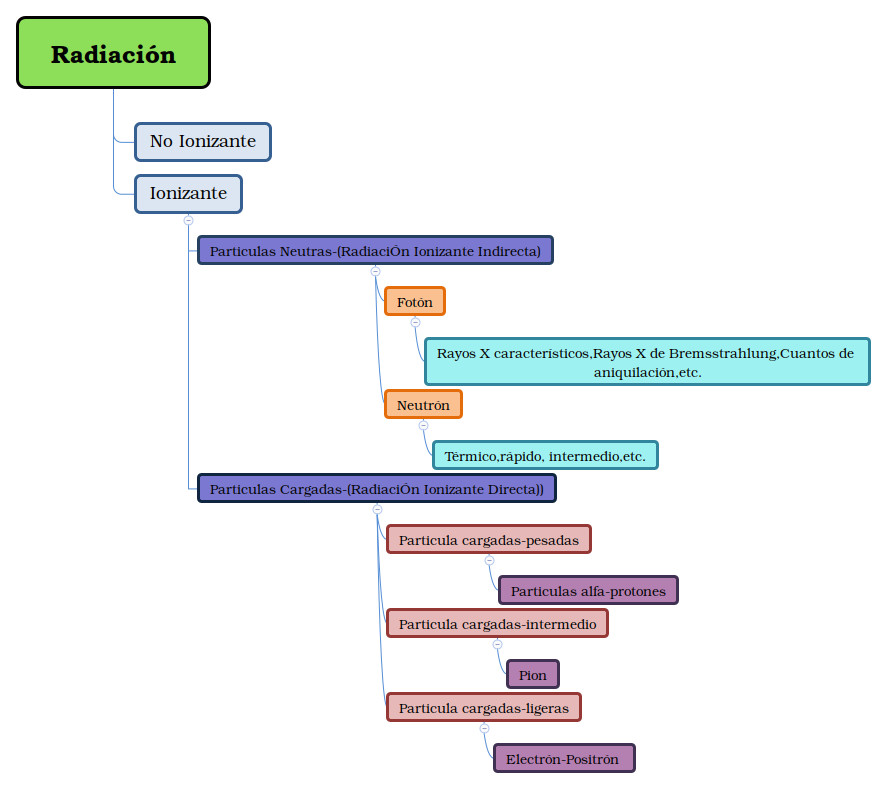
\includegraphics[height=13.5cm]{mapa}
\end{center}

\begin{center}
\begin{itemize}
\item Figura1.0 Clasificación de la Radiación
\end{itemize}
\end{center}

\begin{itemize}
\item \textbf{ Radiación No Ionizante}:Su energía es baja comparada con aquella energía de ionización de los átomos o moléculas de quien absorbe dicha radiación,Ej:Luz visible,ultravioleta, ondas de radio y microondas. 

\item \textbf{ Radiación Ionizante}: Su energía supera el potencial de ionización
de los átomos o las moléculas de quien absorbe.Ej:Partículas alfa ($\alpha$),beta ($\beta$), rayos (x) y gamma ($\gamma$).   



\subsection{Clasificación de  Radiación Ionizante}
Según su clasificación directa o indirecta las radiaciones se emplean en el área de la medicina, para el tratamiento de las enfermedades: en la rama de oncología,radiología,radioterapia, y en el diagnóstico de las mismas en las ramas de imágenes y medicina nuclear con uso de radionuclidos.

 \textbf{Según la forma de ionizar.}%%%%%%%%%%ojo agrandar letra
\item \textbf{ Radiación Ionizante Directa}:Abarca partículas que se encuentran cargadas como los protones, electrones o partículas alpha ($\alpha$)en este proceso de ionizar se involucran las interacciones de Coulomb  entre la partícula que se encuentra cargada y los electrones de los átomos.
\\\\
\item \textbf{ Radiación Ionizante Indirecta}:
 Abarca partículas que no se encuentran cargadas como (\textit{fotones,neutrones o neutrinos}),que cuando atraviesan e interactúan con la materia producen partículas ya cargadas quienes ionizan los átomos y depositan energía  mediante interacciones  de Coulomb con los electrones orbitales de los átomos.
\end{itemize}



\subsection{Clasificación de la Radiación ionizante Directa}
La radiación ionizante directa interactúa con la materia
mediante  la  fuerza  de  Coulomb,lo que causa los electrones de los átomos y moléculas se repelen   o  atraigan
 con respecto a sus cargas.

Se compone de aquellas partículas cargadas:
\begin{itemize}
 \item  Electrones energéticos (Negatrones),
\item Positrones,protones.
\item Partículas  alfa
\item Mesones cargados,muones e iones pesados.
\end{itemize}

\subsection{Clasificación de la radiación de fotones bajo ionización indirecta}
Para el uso especifico en el área de la medicina es importante resaltar algunas de las categorías asociadas a los fotones,en donde una de la tres existentes \textit{ ultravioleta(UV)} tiene uso acotado en los procedimientos médicos llevados a cabo según la especialidad,puesto que en imágenes y tratamientos suelen fotones de energías mayores\textit{(rayos X y rayos gamma ($\gamma$))},
\\

\textbf{ Categorías de los fotones con respecto al origen}
\begin{itemize}

\item Cuantos de aniquilación:Resultan de la aniquilación de positrón y electrón. 
\item Rayos X característicos : Se emiten gracias al uso de  elementos pesados, cuando sus electrones realizan mudanzas entre los niveles más bajos de energía atómica.
\item Rayos gamma($\gamma$): Se obtienen gracias a elementos radiactivos donde se genera una des-excitación de un nucleón de un estado excitado a uno con menor energía o en la descomposición de isótopos radiactivos.

\item Rayos X de Bremsstrahlung: Se generan por interacciones de tipo Coulomb entre el electrón que incidente y el campo nuclear del material.

\item Radiación magnética de bremsstrahlung y ciclotrón:Resulta cuando las partículas cargadas son aceleradas en una trayectoria curva u órbita.

\end{itemize}

%desderevision

\section{Interacción de partículas cargadas con la materia}
 
Al interactuar las partículas con la materia ocasionan efectos que dependen de la clase de partículas,el medio y sus componentes con el que se relaciona.Por el lado de las partículas se tiene en cuenta,masa y carga eléctrica puesto que la interacción es distinta si se encuentran cargadas no.
Aquellas partículas cargadas,principalmente asociado a colisiones coulombianas pierden energía al relacionarse con la materia,colisiones debido a la interacción entre aquellas cargas asociadas a las partículas que inciden y las cargas de protones y electrones de los átomos respectivamente.Estas colisiones se dan por medio de 3 clases de interacciones:
 
                                                                                                                                                                                                                                         
 \begin{itemize}
  \item Colisión inelástica:Las partículas interactúan con los electrones cediendo energía en proporciones pequeñas,dicha energía puede inducir el el elección huya de la atracción del núcleo ocasionando la ionización
  del átomo o en otro caso que el electrón pase de un estado menos ligado excitando al átomo
 
\item Colisión elástica:Las partículas colisionan con los átomo,lo que genera la desviación en su trayectoria,permitiendo así, ceder parte de su energía pero esta vez en términos de energía cinética.Ocasionando la no alteración atómica ni nuclear en el medio.

\item Colisión radiactiva: Razón del fundamento físico de la producción de rayos X,allí se aceleran los electrones que se frenan  bruscamente en un material con un alto número atómico.En esta colisión las partículas cargadas "frenan" o se "desvían" cuando interaccionan con los átomos del medio,lo que permite la emisión de ondas electromagnéticas,osea radiación es comúnmente llamada radiación de frenado.Dicho proceso se da con mayor probabilidad en las proximidades del núcleo atómico gracias a las desviaciones de la  partícula incidente causadas por las cargas eléctricas del núcleo

\end{itemize}

 
 \subsection{Rango de partículas cargadas }
 6.8
 
 Desde el concepto experimental el rango de una partícula que se encuentra debidamente cargada es aquel que suministra el espesor que aquella pueda penetrar,el cual obedece a la masa,la energía cinética,carga de la partícula y estructura del medio.Al penetrar dichas partículas el medio material especifico sufren una serie de colisiones con los átomos que lo componen,pero teniendo en cuenta el espacio vacante relativo en el interior del átomo,aquellas colisiones por choques directos entre los núcleos o electrones y la partícula son muy poco probables.Puesto que como se menciono anteriormente el proceso que sobresale es la colisión culombiana, aquella que se da debido a las fuerzas eléctricas entre la partícula que incide,los electrones y los núcleos del medio. 
 \\\\ 
 Cuando traspasan la materia,aquellas partículas que se encuentran cargadas,en el proceso pierden casi continuamente por radiación y por colisiones ionizantes su energía,sufriendo numerosas deflexiones como consecuencia de la dispersión elástica.Los efectos de esta dispersión se denotan en un porcentaje mas alto para aquellas partículas con carga ligera como los electrones comparado con las partículas de carga pesada ya que ellas no tienen perdidas por efectos de la radiación,puesto que solo transfieren cantidades bajas de energía en colisiones particulares,experimentando desviaciones con ángulos pequeños atribuyéndoles una trayectoria rectilínea.
 \\\\
 Algunos de los rangos de uso cotidiano se relacionan por ejemplo,con la longitud de la trayectoria de una partícula cargada como la distancia total a lo largo de la trayectoria real de la partícula hasta que se detiene,sin importar la  la dirección en la que se mueva,por otro lado,el rango proyectado, se define como la suma de las longitudes de aquellas trayectorias individuales que se proyectan en la dirección de la partícula que incide. 
 
 \section{Produccion Bremsstrahlung}
 
 Dentro de los mecanismos por los cuales existe perdida de energía por medios radiactivos.Existe aquel que experimentan los electrones bajo un campo culombiano pues sufren perdida de energia en forma de espectro continuo mas conocido como radiación de frenado o  Bremsstrahlung.
 
 
El poder de frenado total de aquellas partículas ligeramente cargadas se define como la suma de las ayudas radiactivas y de colisiones como se muestra a continuación:

\begin{equation}
 \left (-  \frac{dE}{dx}\right )_{T}=\left (-  \frac{dE}{dx}\right )_{c}+\left (-  \frac{dE}{dx}\right )_{r}
\end{equation}

Este tipo de producción es de uso considerable en el área de la física médica puesto que la mayor parte de los haz de radiación usados en los procedimientos de radioterapia y radiología se producen por medio de interacciones bremsstrahlung con electrones de un solo valor energético con objetivos solidos,objetivos tales como aceleradores lineales y equipos de rayos x,principales fuentes usadas en estos servicios.

 
Un electrón que golpee con una energía cinética dada a un objetivo especifico sufrirá  distintas interacciones varias con los átomos de dicho objetivo antes de que su energía cinética (Ek) se desvanezca en el mismo.Aquellas interacciones de electrones con un átomo objetivo se describen como:

\begin{itemize}
 \item Cuando incide con el núcleo de un átomo objetivo respectivamente esto produce eventos de dispersión tipo elástica y a su vez puede conseguir una pérdida de radiación acompañada de la producción de bremsstrahlung.
 \item Al existir una interacción del electrón incidente con el electrón orbital de un átomo objetivo esto provoca inicialmente una pérdida por impacto de colisión y la ionización del átomo objetivo quien puede estar  acompañada de un electrón con energía definido como rayo delta.Luego de la pérdida de colisión en un objetivo de rayos X esta es seguida por una  emisión de rayos X característicos y electrones de Auger.
 Electrones de Auger que se denominan como aquel proceso en el cual los electrones con ciertas energías características son despedidos de los átomos,respondiendo a la mudanza descendente de otro electrón del átomo.
 \end{itemize}

 Aquella intensidad máxima perteneciente a los rayos X se producen en un ángulo peculiar $\theta$ max,el cual depende de la energía cinética de los electrones incidentes;

\begin{itemize}

\item 
 En el rango de energía de diagnostico (50 kVp a 350 kVp), los tubos de rayos X se utilizan para la producción de rayos X y la mayoría de los fotones se emiten a $ 90\textdegree$ desde la dirección de desaceleración de electrones en el objetivo.El ángulo característico $\theta$ max es igual a $90\textdegree$.



\item
 En el rango de radioterapia de mega voltaje (4 MV y superior), las guías de onda de aceleración se utilizan para la aceleración de electrones y la producción de rayos X,la mayoría de los fotones se emiten en la dirección de desaceleración de electrones en el objetivo. El ángulo característico $\theta$ max es entonces  $\sim 0\textdegree$ y el objetivo se conoce como de transmisión.

Aquellos haces de rayos X que se producen en los objetivos de rayos X son distintos y contienen fotones de varias energías que van desde $0$ hasta un h$\nu$ max de energía máxima que es equivalente a la energía cinética de los electrones,quienes golpean al objetivo.


%*Tomado de(ojo,citar) 

 \end{itemize} 
 
 
\section{Interacción materia-energía \textit{(fotones)}}

Los fotones son partículas diminutas a quienes se les atribuye el transporte de energía en forma de radiación,son capaces de estimular electrones de los átomos logrando así el salto a orbitas de nivel superior,sin dejar de lado la característica de incitar la ionización de aquellos átomos.Donde parte de esa energía asociada a los fotones que inciden se usa para transmitir la energía cinética Ek a aquellos electrones propios del material.

Si tenemos  fotones con un solo valor energético en un haz e inciden sobre cierto material con espesor característico, si se deseara medir cuantos de ellos logran atravesar el material e impactar con el detector,se pueden dar eventos u opciones tales como:

\begin{itemize}
 \item Las partículas traspasen cierta parte de energía y al chocar cambien su dirección,logrando que el detector en su medición encuentre menos cantidad de fotones, a lo que se le atribuye en nombre de atenuación,fenómeno que involucra los efectos de  procesos como la dispersión y absorción de dichas partículas.
 \item Las partículas sigan su trayectoria,logren atravesar el material y sin que exista ninguna interacción lleguen al detector.
 \item Las partículas interactúen con el medio,entreguen energía en su totalidad al material evitando la llegada de las partículas\textit{(fotones)}al detector.
 \end{itemize}


 Debemos recordar que los fotones hacen parte de la radiación de tipo indirectamente ionizante,debido a que  cuando interactúa con la materia  provoca ionizaciones,allí es donde únicamente aquellos fotones que son absorbidos transfieren al medio su energía.Mientras que otros de ellos,quienes interactúan con el medio,logran desviarse de la trayectoria sin ceder energía pero si dispersándose.
 
 
Aquellos  procesos donde los fotones interactúan con la materia obedecen a los siguientes aspectos:
\begin{itemize}
 \item Energía de la radiación que incide.
 \item Tipo de material donde la radiación incide.
\end{itemize}

\subsubsection{Interacciones fotónicas de importancia en el área de física médica }

\begin{itemize}
 \item Física presente en la atenuación y dispersión de haces de fotones en tejidos de importancia,imágenes y dosimetría de radiación.
 
 
\item Necesario e importante en dosimetría de radiación:todos los aspectos físicos que se involucren en los procesos de:planificación del tratamiento, suministro de dosis y prescripciones de dosis en procedimientos clínicos.

\item  Física presente en la transferencia de energía de fotones a partículas cargadas de luz en un absorbente y absorción de energía  en tejidos. 

\item Física presente en  la producción de neutrones:Seguimiento,planificación y evaluación de los procedimientos específicos en estos proceso puesto que representa un peligro potencial para la salud de los pacientes y el personal involucrado con el uso de linacs de alta energía.
\end{itemize}


\subsection*{Efecto Fotoeléctrico}
En este fenómeno existe una emisión de electrones provenientes de las superficies de los metales cuando incide luz sobre las mismas,los electrones emitidos llevan consigo una Ek máxima la cual no depende  
de la intensidad de radiación que incide,siendo esta una de las principales características del fenómeno seguido de:

\begin{itemize}
 \item Los fotones cuentan con una energía proporcional a la frecuencia de la onda que se le asocia.
 
 La Ek max que se obtiene depende solo de $\nu$(frecuencia de la radiación que incide).
 \item Existe intercambio de energía entre radiación-materia siempre y cuando se realice en múltiplos de un cuanto de energía.
 \item Un electrón en reposo absorbe un fotón de energía Ef = h$\nu$ ($\nu$frecuencia de la onda y h la constante de Planck). 
 
 \item Existe una emisión de electrones y una transferencia de energía fotón-electrón instantánea.
\end{itemize}

\begin{center}
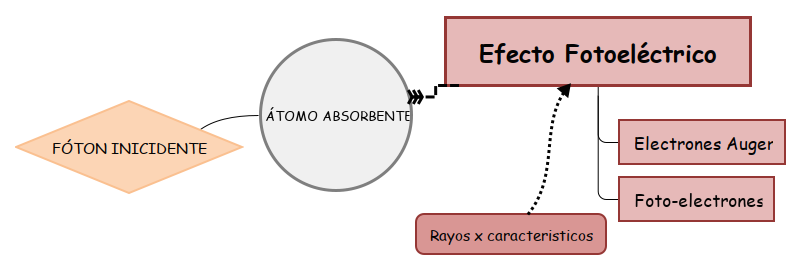
\includegraphics[height=5.5cm]{ef}
\end{center}


\subsection*{Producción de Pares (Electron-Positron)}

Esta es una de las formas en la que los fotones interactúan con la materia siempre y cuando ellos tengan una energía (E=h$\nu$) mayor que la energía de masa de un electrón en reposo mas  un positrón.

\begin{itemize}
 \item Considere que la energía de masa en reposo del electron es de 0,511 MeV y para que exista una interacción de producción de pares la energía debe ser igual o mayor que 1,022MeV.
\end{itemize}


La energía de masa en reposo del electrón es 0,511 MeV, así que por encima de 1,022MeV de energía fotónica, es posible la producción de pares. Para energías de fotón muy por encima de este umbral, la producción de pares se convierte en el modo dominante de la interacción de los rayos X y los rayos gamma con la materia.
\begin{center}
\includegraphics[height=5.5cm]{pr}
\end{center}


\subsection*{Efecto Compton }
En este fenómeno cuando la radiación electromagnética incide sobre las superficies la longitud de onda a salir es mayor con respecto a los valores con los que ingreso.

\begin{center}
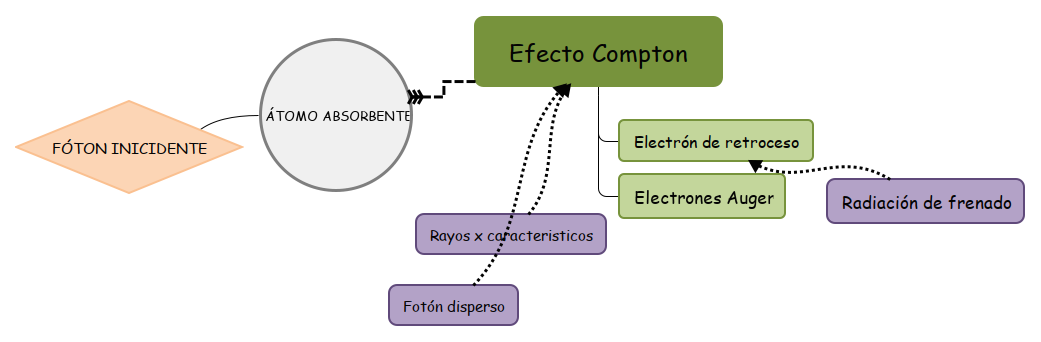
\includegraphics[height=5.5cm]{com}
\end{center}

\subsection{Interacción en un absorbente} 
En este caso los fotones al atravesar el medio material consiguen sufrir interacciones varias con los átomos propios del medio,interacciones que implican a los electrones o cualquier núcleo del medio en si

Aquellas interacciones con los núcleos se pueden dar directamente fotón-núcleo a lo que se denomina\textit{foto desintegración } o por otro lado se puede dar interacciones entre el campo electrostático del núcleo y el fotón,proceso llamado\textit{ producción de pares}.
\\\\
Cuando se generan interacciones fotón-electrón, se atribuye a que se den por Efecto Compton,Dispersión de Thomson,Efecto Fotoeléctrico o dispersión de Rayleigh.Procesos que se relacionan mas adelante.



Para estimar lo que sucede con el fotón luego de interactuar con la materia,existen dos posibles eventos:

\begin{itemize}
 \item El fotón se dispersa con dos posibles eventos:El fotón que se efectúa contiene la energía equivalente del fotón que insidio causando la no liberación de partículas cargadas con luz en la debida interacción y entro del otro evento posible se contempla,aquel fotón dispersado contiene una energía en proporciones bajas con respecto al fotón incidente,pero aquella energía se encuentra en exceso se cede a un electrón  
 
 \item El fotón se extingue absorbiendose totalmente permitiendo que una fracción de su energía se traslade a partículas cargadas de luz tales como positrones o electrones.  
\end{itemize}

Estas partículas cargadas \textit{positrones y electrones} que se producen o se liberan en el medio gracias a las interacciones relacionadas con los fotones,pueden consignar energía en el medio mediante interacciones de Coulomb con electrones proceso conocido como perdida de ionización o pueden irradiar  energía cinética Ek en forma de fotones también mediante interacciones de Coulomb con los núcleos del medio proceso llamado pérdida de radiación.
\\\\
A continuación se muestra algunas relaciones físicas relacionadas  con el tema en mención.

{%
\newcommand{\mc}[3]{\multicolumn{#1}{#2}{#3}}
\begin{table}[h!]
\begin{center}
\begin{tabular}{|c|c|c|c|c|}\hline
\rowcolor{ocre!40}
\textbf{Cantidad} & \textbf{Definición} & \textbf{Unidad} & \textbf{Conversion} & \textbf{Aspectos} \\\hline



\textbf{Exposición (X)}
& %X=\frac{\Delta Q}{\Delta m _{air}}
%2.58 \cdot  \frac{10^{-4} C}{kg_{air}}% 
X & 2 & %1R=2.58 \cdot  \frac{10^{-4} C}{kg_{air}} 
1
&    \mc{1}{c|}
%{\Delta Q \Delta m _{air}%
{Suma de todas las cargas electricas de los iones de un signo producidos en aire-
Masa de aire }\\\hline %{\Delta Q - \Delta m _{air}}%\\\hline
\textbf{Kerma (K)}
& 
%K=\frac{\Delta E_{tr}}{\Delta _{m}}
k &
%1Gr=1\frac{J}{kg}
1 & / & \mc{1}{c|}{/}\\\hline
%/\Delta E_{tr}
%/ \Delta _{m}
\textbf{Dosis (D)} & 
%D=\frac{\Delta E_{ab}}{\Delta _{m}}
D & 1
%1Gr=1\frac{J}{kg}
& 1Gy=100rad
& \mc{1}{c|}{Energía depositada-Unidad de masa}\\\hline
%\Delta E_{ab}
%\Delta _{m}
\textbf{Dosis Equiv (H)} & H
%H=D\omega_{R}
& 1 Sv & 1 Sv=100 rem & \mc{1}{c|}{D$\omega$R:Dosis multiplicada por un factor de ponderación de la radiación}\\\hline
%\omega_{R}

\textbf{Actividad (A)} & A
%A=\lambda N
& 1
%1 Bq=1s^{-1}
& Bq 
%1Bq=\frac{1Ci}{3.7\cdot 10^{10}}
& \mc{1}{c|}{Bq:becquerel.
Ci:Curie.

$\lambda$Constante decaimiento:N}\\\hline
\end{tabular}
\caption{Medidas y unidades de radiación.}
\label{table:1}
\end{center}
\end{table}

Dentro de  radiación ionizante  entran como una de las categorías los fotones energéticos los cuales pueden interactuar con la materia de formas distintas.


{
%\newcommand{\mc}[3]{\multicolumn{#1}{#2}{#3}}
\begin{table}[h!]
\begin{center}
\begin{tabular}{c}\hline
\rowcolor{ocre!70}
\mc{1}{|c|}{\textbf{Interacción}}\\\hline
\mc{1}{|c|}{\textit{Dispersion de Thomson}}\\\hline
\mc{1}{|c|}{\textit{la dispersión de Rayleigh}}\\\hline
\mc{1}{|c|}{\textit{Dispersion Compton}}\\\hline
\mc{1}{|c|}{\textit{Efecto fotoeléctrico}}\\\hline
\mc{1}{|c|}{\textit{Producción de pares nucleares.}}\\\hline
\mc{1}{|c|}{\textit{Producción triplete}}\\\hline
\mc{1}{|c|}{\textit{Fotodisintegración}}\\\hline
\end{tabular}
\caption{Posibles interacciones radiación-materia en los fotones.}
\label{table:1}
\end{center}
\end{table}
}%

\begin{itemize}
 \item Las probabilidades de interacción radiación-materia con fotones,dependen de la energía del fotón incidente  h$\nu$ y del número atómico Z del absorbedor.
\end{itemize}

 Dentro del área de física médica y dosimetría de radiación, las interacciones de los fotones con el átomo del absorbente se clasifican de la siguiente manera según su nivel de importancia:

\begin{itemize}
 \item Interacciones de los fotones con el átomo del absorbente
\end{itemize}


\begin{center}
\begin{tabular}{|c|c|}\hline
\rowcolor{ocre!70}
\textbf{Interacciones de mayor importancia} & \textbf{Importancia Moderada}\\\hline
Efecto fotoeléctrico. & Dispersión de Rayleigh\\\hline
Dispersión compton por electrón "libre". & / \\\hline
Producción de pares en el campo del núcleo  y  producción de tripletes. & / 
\\\hline
\end{tabular}
\end{center}

\begin{center}
\begin{tabular}{|c|c|}\hline
\rowcolor{ocre!70}
\textbf{Menor importancia} & \textbf{Interacciones insignificantes}\\\hline
\textit{Efecto fotonuclear.} & \textit{Dispersión de Thomson por el núcleo.}\\\hline
\textit{Dispersión de Thompson por electrón "libre".} & \textit{Compton que dispersa por el núcleo.}\\\hline
\textit{/} & \textit{Producción de mesones.}\\\hline
\textit{/} & \textit{Dispersión elástica de fotones por la producción de pares nucleares virtuales en el campo de Coulomb nuclear.}\\\hline
\end{tabular}
\end{center}


\section{Interacción de partículas cargadas}
 Los átomos inicialmente se encuentran neutros eléctricamente hablando.En este proceso cuando una partícula que se encuentra cargada golpea un electrón orbital lo expulsa del átomo, lo que ocasiona la formación de un par de iones.Puesto que la eliminación de este electron del átomo disminuye el numero total cargas negativas por uno, deja el átomo con una carga positiva,y este ion par consiste en:
 
 \begin{itemize}
\item El átomo cargado positivamente
\item El electrón cargado negativamente
Y son estas partículas que de esta manera son  capaces de crear pares iónicos a quienes se les llama radiación ionizante. 
 \end{itemize}
Son las partículas cargadas (beta y alfa) los tipos mas comunes dentro de la mayor parte de las aplicaciones,interacciones que se tratan a continuación.


\subsection{Partículas Alfa}
Esta partícula es un núcleo de helio que ha sido desprendido de sus electrones orbitales, se emite desde un átomo radiactivo con una velocidad de aproximadamente 1/20 de la velocidad de la luz y con energías entre 4 a 9 MeV.Dichas partículas provocan ionizaciones en la materia cuando son desviados por la carga positiva de un núcleo y arrastran los electrones orbitales (atraídos por la carga positiva del alfa) junto con ellos,estas partículas desencadenan excitaciones a lo largo de su trayectoria al  
atraer electrones orbitales internos hacia órbitas externas.Es así como se da energía
fuera del átomo como radiación fluorescente o rayos X de baja energía, cuando los electrones vuelven a caer en las vacantes orbitales internas.

Ya que las partículas alfa tienen una masa relativamente grande (2 neutrones y 2 protones), una carga eléctrica alta (2+) y baja velocidad, creando muchos pares de iones en una longitud de camino muy corta
a lo que llamamos ionización específica que por la característica anteriormente mencionada es muy alta y es esta la razón por la cual  pierde toda su energía en una distancia muy corta.

Su alcance en el medio (aire) es de algunos centímetros, incluso para las partículas alfa con energías  considerables.Considerando el rango limitado en materia,esta no presenta peligro de radiación externa para el ser humano.

Muchas partículas alfa no pueden penetrar la capa protectora de la piel.En el caso de que se presente lo contrario e ingrese al cuerpo, rodeado de tejidos vivos, el daño será en el área local en la que se deposita este emisor alfa.Es por esto que a nivel interno son peligrosas y debe evitarse la ingesta. 
 

\subsection{ Partículas Beta}
Estas partículas se emiten desde el núcleo de un átomo con naturaleza radiactiva
con un rango amplio de energías hasta un valor máximo.En el caso cuando se emite una beta que está por debajo de este valor máximo, el neutrino se lleva el resto de la energía.

Dichas partículas beta,igual que las partículas alfa, pierden su energía por ionización y excitación, su masa (1/7300 de un alfa)sigue siendo muy pequeña y contiene una carga baja aproximada de (1/2 de la de un alfa),es por esto que las interacciones tienen lugar en intervalos menos frecuentes.Estas partículas beta no producen muchos pares de iones por centímetro de trayectoria como las partículas alfa y, por esta razón, tienen un alcance mayor en la materia. Este rango de la partícula beta en la materia depende de su energía y la composición especifica del material.

\begin{itemize}
 \item Producción de rayos X de Bremsstrahlung:
Para este caso en particular las partículas beta pueden interactuar con el núcleo de un átomo y dar lugar a rayos X, método llamado Bremsstrahlung (Radiación de frenado),que sucede cuando una partícula beta de velocidad alta. La interacción eléctrica que se da entre la partícula beta negativa y el núcleo cargado positivamente hace que ocurra la desviación de la partícula beta de su camino original deteniéndose  por completo,esta desviación causa un cambio en la velocidad  de la partícula beta con la emisión de rayos X de diversas energías. Las probabilidades de producción de Bremsstrahlung aumenta con el aumento del número atómico del absorbente,dichas partículas (beta) posees una energía de más de 70 keV para lograr penetrar la capa que protege la piel y es la razón por la cual representan un peligro externo. Pero a su vez la partícula beta también puede constituir un peligro interno,esta partícula tiene un mayor rango en el tejido en comparación con la partícula alfa debido a su baja ionización específica, por esta razón, entrega menos energía por unidad de volumen de tejido,siendo no tan efectiva para causar daño como una partícula alfa.
\end{itemize}

\subsection{Interacción de rayos X y rayos gamma}
En términos de protección radiológica los rayos X y los rayos gamma son idénticos, difieren únicamente en su lugar de origen. Aquellos rayos gamma se emiten con energías discretas desde los núcleos que se encuentran excitados.Estos rayos X se emiten desde fuera del núcleo; es decir, un electrón de capa externa reemplaza a un electrón de capa inferior faltante y se produce una radiografía característica, o la interacción de partículas beta hace que se produzca la radiación de Bremsstrahlung. 

La energía que maneja un rayo X característico es aproximadamente igual a la diferencia en los niveles de energía de los electrones, pero la radiación Bremsstrahlung produce un espectro continuo de energías hasta un valor máximo.Esos rayos X $\gamma$ no tienen carga, tampoco interactúan por fuerzas electrostáticas como en el caso de partículas cargadas, que causan la ionización de la materia directamente a lo largo de su recorrido.Aún así los rayos X y gamma tienen suficiente energía para liberar partículas cargadas secundarias (los electrones) de la materia a través de una de tres interacciones básicas: 

\begin{itemize}
\item Efecto fotoeléctrico
Interacción de fotones de rayos X o $\gamma$ , así como otros fotones(la luz), por lo que toda la energía del fotón se transfiere a un electrón de capa interna (casi siempre la capa K), expulsando el átomo y dejando el átomo con una vacante de caparazón interior. Esta vacante de caparazón crea una energía de excitación que corresponde a la energía de unión (BE) del fotoelectrón expulsado.

\item Efecto Compton 
Los fotones con energías mucho mayores que la energía de union (BE) de los electrones en un átomo pueden interactuar a través de interacciones de dispersión en las que se conserva la energía cinética %KE
total del sistema. En esta interacción, el electrón aparece al fotón como un electrón libre,donde su energía  de union es igual a 0,(BE = 0).

En este proceso, el fotón disperso y el electrón Compton comparten la energía del fotón incidente (gamma).Le energía cinética (KE) llevado por el electrón Compton puede depositarse localmente,osea,ser absorbido de manera inmediata por el entorno).Aun así, la energía transportada por el fotón disperso Compton no se deposita localmente. Por lo tanto, este fotón disperso puede contribuir significativamente a la dosis fuera de un aparato de protección.

\item Producción en pares.
Los fotones gamma($\gamma$) de alta energía transpasan su energía principalmente por producción de pares. Un haz de rayos X o gamma de energía  alta que pasa cerca de un núcleo desaparece 
súbitamente,es allí cuando un electrón y un positrón aparecen en su lugar. Esta interacción debe tener lugar en un campo eléctrico, generalmente el del núcleo, para conservar el impulso o momentum.

Dado que ambas partículas se crean a partir de la energía proporcionada por el fotón que incide, el proceso es posible energéticamente hablando, solo si $E_{\gamma}$es mayor que 1.022 MeV, que es la suma de la energía de masa en reposo de un electrón y un positrón (0.511 MeV cada uno).

\begin{itemize}
\item  Energía de masa en reposo que se denomina como la cantidad de energía que se liberaría si una partícula de masa m se convierte en energía,viendolo posible si recordamos la famosa teoría de Einstein de que $E = mc^{2}$,
dónde:

\subitem E = energía de fotones (en julios, se puede convertir a MeV)
\subitem  m = masa en reposo de dos electrones (en kilogramos)
\subitem  c = la velocidad de la luz $(3 x 10^{8}$ m / seg)
 
Cuando el positrón se pone mas lento, perdiendo su energía cinética, se somete a la aniquilación del positrón combinándolo con un electrón. Esto produce dos fotones con energías de 0.511 MeV cada uno, emitidos a 180$^{o}$ uno del otro. Esta "radiación de aniquilación" representa la energía de masa en reposo de dos electrones, que se convierte en energía en su máxima expresión en forma de fotones.

\end{itemize}
\end{itemize}

\section{Cantidades unidades de Radiación}
Es de gran importancia comprender las distintas cantidades y unidades que se utilizan al referirse a la radiación,junto con las unidades que al transcurrir el tiempo han cambiado. 


\subsection{Tasa de conteo}
Se define como el número,la cantidad de interacciones de radiación que ocurren en el detector en un período de tiempo determinado. Esta medida se trabaja en unidades como cps (conteos por segundo) o cpm (conteos por minuto). Es mas útil para medir la radiación de partículas, aunque tambien puede usarse para pequeñas cantidades de rayos X o radiación gamma.

Es común ver la tasa de conteo medida en dps (desintegraciones por segundo) o dpm (desintegraciones por minuto), aunque esta no es realmente una tasa de conteo real. Las mediciones trabajadas en dps o dpm han tenido en cuenta la eficiencia de los detectores para para lograr estimar la verdadera tasa de desintegración.

\subsection{Exposición}
Se establece como la medida de la cantidad de carga eléctrica que producen  los fotones en una masa de aire.Esa carga eléctrica proviene de la producción de pares de iones, que el detector recoge y mide como corriente. Se puede medir como una tasa (exposición por unidad de tiempo), para aquellas fuentes que emiten radiación continuamente, o como una exposición integrada total, para fuentes como tubos de rayos X que emiten radiación en un solo pulso.

La unidad tradicional utilizada para la exposición es el roentgen (R). 1 R es la cantidad de radiación requerida para liberar una unidad de carga electrostática (de cualquier signo) en 1 $cm^{3}$ de aire a temperatura y presión estándar (STP).  Esto equivale a aproximadamente 2.08x$10^{9}$ pares de iones. En unidades SI,1R=2.58 x 10 $^{-4}$ C / kg.

\subsection{Dosis absorbida}
Se establece como medida de la energía que se deposita en un material por todos los tipos de radiación. La unidad tradicional es el rad (dosis de radiación absorbida), que es igual a 100 ergios / gramo. La unidad SI para la dosis absorbida es el grey (Gy), igual a 1 joule / kg. 1 Gy = 100 rads.

Es difícil de medir directamente, por lo que es frecuente que se calcule a partir de otras cantidades, como la exposición. Para calcularla, es necesario conocer el factor de conversión correcto para el material de interés.Se debe tener en cuenta que en la protección radiológica, el roentgen y el rad con frecuencia se usan indistintamente ya que, en el tejido, son aproximadamente iguales. Aun así el roentgen es una unidad de exposición y se aplica solo a las radiaciones x o gamma.

\subsection{Dosis equivalente}
\textquotedblleft HT \textquotedblright es una cantidad calculada a partir de la dosis absorbida que tiene en cuenta que algunos tipos de radiación son más nocivas para el tejido biológico que otros. Es igual a la dosis absorbida en un tejido de cada tipo de radiación $(D_{R,T})$ multiplicada por un factor de ponderación de radiación $(W_{R})$ para ese tipo de radiación, sumado a todos los tipos de radiación presentes:

\begin{equation}
 H_{T}=\sum_{R} W_{R} X  D_{R,T}
\end{equation}

La unidad aconstumbrada utilizada para la dosis equivalente es el rem. La unidad SI es el sievert (Sv), y 1 Sv = 100 rem. El factor de ponderación de la radiación no tiene unidades; sin embargo, se usa una unidad diferente para la dosis equivalente para que sea fácilmente distinguible de la dosis absorbida.

\subsection{Dosis efectiva}
Esta cantidad  tiene en cuenta que los diversos órganos y tejidos del cuerpo humano responden a la radiación de manera distinta. Se usa principalmente en protección radiológica, y está destinado a comparar el riesgo de efectos estocásticos asociados con una exposición no uniforme a la radiación con el de una exposición uniforme en todo el cuerpo. 

\footnote{ Un efecto estocástico es un efecto sobre la salud que ocurre al azar y para el cual la probabilidad del efecto se supone que ocurre, en lugar de su gravedad, como una función lineal de la dosis.}
La DE se calcula multiplicando la dosis equivalente (HT) para cada órgano / tejido por el factor de ponderación de tejido para ese órgano / tejido (wT), sumado a todos los órganos / tejidos del cuerpo:

\begin{equation}
H_{T}=\sum_{T} W_{T}   x    H_{T}
\end{equation}
Esta variable sigue siendo medida en rem o sievert.

\subsection{Dosis efectiva comprometida}

La CED o CEDE es una cantidad que calcula la dosis total que un sujeto recibiría durante toda la vida de una ingesta de material radiactivo. Se debe tener en cuenta que la tasa de dosis generalmente disminuye con el tiempo, dependiendo de la vida media de la sustancia y la velocidad a la que el cuerpo lo elimina.
\subsection{Dosis efectiva total}

Es básicamente igual a la suma de la dosis de radiación  externa más la dosis de radiación interna:
\begin{equation} 
TED = ED + CED
\end{equation}
%libr

%Por esta razón, los escudos beta están hechos de materiales de bajo número atómico, como aluminio o plástico, para reducir la producción de Bremsstrahlung. Los tubos de rayos X están hechos con materiales de alto número atómico, para fomentar la producción de Bremsstrahlung.

%%%%




\subsection{Parámetros físicos del haz de radiación a utilizar en un tratamiento}

La selección del haz de radiación y debida  prescripción de dosis para el tratamiento con radiación según el tipo de afección debe obedecer a ciertos factores  ejemplo de ello son aquellos que tienen injerencia con la física,por ejemplo:

Según el diseño de la maquina,energía del haz,dosis de profundidad,tamaño,entre otros.
• Densidad de la ionización que se produce en el tejido a causa del haz de radiación usado en el tratamiento.%\cite{libro}page25%

\section{Propiedades de la Radiación Electromagnética}

Recordemos que cuando tratamos con cargas eléctricas inmóviles estas producen campos eléctricos,pero cuando las cargas se encuentran en movimiento,producen campos eléctricos y a las vez magnéticos que cuando sufren cambios regulares y recurrentes producen RM \textit(Radiación Electromagnética) quien permite conducir energía.Cuenta con las siguientes características:
\\
\begin{itemize}
 \item No contiene posee masa en estado de reposo
 \item Transmite una energía hf con longitud de onda $\lambda$ y momento pv=h/$\lambda$,siendo h la constante de Planck.
\end{itemize}
Cuando se trata de la liberación de un electrón en un metal se necesita una mínima energía según el material, denotada como la función trabajo $\phi$, teniendo en cuenta esto, Einstein formula que debe existir una energía cinética máxima                                                                                                                                                                                                                                           (Ek) con la que el electrón es despedido de la superficie del mismo por un fotón con energía hf,expresada de la siguiente manera:
\begin{equation*}
 E_{k}=hf-\phi
\end{equation*}

Donde la $\Phi$, es la cantidad mínima de energía necesaria requerida para estimular fotoemisión de electrones en la superficie de un metal,quien también depende de las características del mismo,estimando la no dependencia con la intensidad  radiación que incide.

Es importante recordar a partir de lo antes mencionado que a aquella emisión de electrones en las superficies metálicas se le conoce como \textbf Efecto Fotoeléctrico

HASTA AQUI!




\subsection{Influencia de la geometría en la determinación de coeficientes de atenuación}


$\bm \mu $ Coeficiente de atenuación, el cual se establece de  manera experimental a partir de la técnica de geometría de \textit{haz estrecho} que comprende una fuente de fotones de una sola energía colimados estrechamente y un detector igualmente colimado.

Para un medio indiferenciado, este coeficiente de atenuación  $\mu$ es constante u uniforme,deduciendo así la siguiente relación Matemática,valida para haces de fotones con una sola energía.

\begin{equation}
I={I(X)}= I(0)e^{-\mu x}
\end{equation}



\begin{itemize}
 \item 
Cuando se hace uso de un haz extenso o amplio en términos geométricos para establecer coeficientes de atenuación y secciones transversales en la atenuación del haz de fotones,en este caso la lectura disminuye gracias a la disminución del haz primario en el absorbedor y se incrementa por la radiación que se dispersa desde el absorbente hacia el detector especifico.


El factor de acumulación que permite interpretar aquellos fotones secundarios que se dispersan desde el absorbente hacia el detector se define como:

\begin{equation}
 B=\frac{I_{B}(X)}{I_{N}(X)}
\end{equation}

\begin{itemize}

\item  Donde ${I_{B}(X)}$ es la señal medida por el detector para un espesor del absorbedor especifico cual sea en geometría de haz amplio ancho.
 \item ${I_{N}(X)}$ 
 es la señal de geometría de haz estrecho para el espesor del absorbedor especifica. \end{itemize}
\end{itemize}


\section {Detectores de Radiación Ionizante}

Es importante generar  medidas efectivas para estimar  dosis apropiadas en un procedimiento médico,lo que se conoce comúnmente como \textit {dosimetría} ya sea para preparar las áreas físicas donde se realizaran los procesos o la estimación de dosis en trabajadores ocupacionalmente expuestos,según sea el caso se referencia como: \textit{Dosimetría de área y Dosimetría personal}

En la área de radiología el personal a cargo de la protección radiológica es el encargado de clasificar a los trabajadores, según el riesgo de exposición a radiación ionizante para así,
instaurar medidas de control por medio de la vigilancia dosimétrica, individual o del ambiente de trabajo según sea el caso.

Para realizar una debida tasación de dosis en tejido asociado a la piel se puede determinar haciendo uso de dosímetros de termoluminiscencia o cámaras de ionización.Los TLD \textit{dosímetros termoluminiscentes}gracias a sus pequeños tamaños posibilitan la ubicación sobre el cuerpo de la persona obteniendo una medida de la radiación difusa,mientras que las cámaras de ionización gracias a su tamaño mucho mas considerable que el dosímetro no es colocado cerca de la piel.Estos son algunos de los casos donde es mas que necesario el uso de detectores para detectar la presencia de
un campo de radiación ionizante en procesos médicos puesto que no es percibida mediante los sentidos u órganos del ser humano, una de las razones por las cuales es necesario hacer uso de ellos como dispositivos de detección para tener un porcentaje alto en protección radiológica.
 
Cuando la radiación interactúa con la  materia esta transfiere energía,generando efectos posibles de medir,tales como: Alteraciones biológicas,excitación de luminiscencia en solidos,ionización de la materia o de gases.



Los detectores de radiación ionizante son dispositivos que se ubican en un medio donde existe un campo de radiación,se constituye de un  material sensible a este tipo de energía radiación y un sistema que transforma dichos efectos en un valor correspondiente a la lectura.En seguida se describen aquellos detectores que podemos encontrar en el servicio de radiología:

\begin{itemize}
 \item Cámaras de ionización:EStos dispositivos recogen las cargas que son liberadas por las radiaciones cuando ionizan un gas,dichas cargas se recolectan mediante un par de electrodos  entre los que existe una diferencia de potencial parar no permitir se produzca  el fenómeno de la recombinación.(Detección para niveles de radiación mayores a 1 mR$/$h,eficientes en la de detección partículas alfa o beta)
 
 \item Contador proporcional:Para poder evidenciar pulsos individuales, es necesario aumentar el voltaje por arriba de los 1000V, así el campo eléctrico acelera los electrones y estos generan ionizaciones secundarias,aquellos electrones secundarios acelerados producen nuevas ionizaciones que generan cascada de ionizaciones,detectando la llegada de la partícula inicialmente pero no su energía.Se usa para  la detección de rayos X y electrones de baja energía.

 
 \item Contador Geiger-Muller: Es un detector de ionización, que funcionan gracias a una alta tensión en una determinada región en donde por un solo evento se crea un pulso de avalancha.Detección de niveles bajos de radiación.
 
 
 \item Detector de centelleo:Consta de una sustancia que emite luz cuando es golpeada por una partícula ionizante.Utilizado principalmente para formación de imágenes(gammagrafia).
 
 
\item Estos dispositivos miden dosis en regiones donde la 
existen variaciones significativas debido a la región de la acumulación de un haz de alta energía.(Usado en la Monitorización personal)  
\end{itemize}


 

\section{Protección Radiológica}

La protección radiológica tiene como fin garantizar los cuidados óptimos de  personas y del medio ambiente contra aquellos efectos perjudiciales que puede acarrear la exposición exposición a radiaciones de tipo ionizante.



Mediante acciones o actividades tales como;sistema de rayos X en aplicaciones médicas de Radio diagnóstico como radiología dental o tomografía computarizada e intervencionismo, existe una exposición a la radiación ionizante ocupacionalmente hablando,niveles de exposición que se necesitan evaluar y cuantificar ya que este campo (salud) contribuye en gran parte la exposiciones de una población en general.
 
Es por esto que entidades como la Comisión Internacional de Protección Radiológica establecen normas y sugieren recomendaciones en la aplicación de técnicas radiológicas que beneficien a la población evitando el mayor riesgo posible en la dosis de exposición ocupacional.
Es importante tener en cuenta que debe existir respectivamente una razón clínica con visto bueno que por lo menos estimule en llevar a cabo el procedimiento con mas beneficios que riesgos para el paciente o trabajador expuesto,luego de que se justifique médicamente la practica, esta debe convenir la dosis mas baja que se pueda mediante una proceso determinado de optimización.
\\\\
Los límites de dosis para trabajadores expuestos a radiaciones ionizantes en Colombia es tan relacionados de la siguiente manera:

{%
%\newcommand{\mc}[3]{\multicolumn{#1}{#2}{#3}}
% \definecolor{tcA}{rgb}{0,1,1}
%\definecolor{tcB}{rgb}{0.666667,1,1}

\begin{table}[h!]
\begin{center}
\begin{tabular}{|c|c|}\hline
\rowcolor{ocre!70}
\mc{2}{||c||}{\textbf{Exposición a Radiaciones Ionizantes}}\\\hline
Tipo de Exposición  & Limite\\\hline
\rowcolor{ocre!40}
\mc{2}{|c|}{\textbf{Dosis equivalente al año 
en}}\\\hline
Piel& 500 mSv\\\hline
Cristalino& 150 mSv\\\hline
\rowcolor{ocre!40}
\mc{2}{|c|}{\textbf{Dosis efectiva }}\\\hline
Un año  & 50 mSv \\\hline
Promedio en 5 años & 20 mSv \\\hline
\end{tabular}
\caption{Valores establecidos de exposición de radiación ionizante según la comisión internacional de protección radiológica.}
\label{table:1}
\end{center}
\end{table}

}%
Recordemos que para lograr obtener mediciones de la dosis de radiación ionizante y conocer si existe algún tipo de  daño biológico es imprescindible 
disponer  de magnitudes y  unidades óptimas tales como;
\begin{itemize}
 \item 
Dosis efectiva: Dosis equivalente ponderada por el factor de ponderación de tejido.Sievert(Sv)-Julio/kilogramo.(1 Sv(SI) = 100 Rems). 
\item 
Dosis equivalente: Dosis absorbida ponderada por el factor de ponderación de la radiación. Sievert (Sv)-Julio/kilogramo.
\item 
Dosis absorbida:Energía absorbida por unidad de masa. Gray (Gy)-Julio/kilogramo.(1Gy(SI)equivale a 100 rads)
\end{itemize}

Con respecto los datos tenidos en cuenta como limite de exposición a la radiación,es necesario revisarse mínimo una vez al mes los datos que reportan los instrumentos de medida respectivamente \textit{Dosímetros} y evaluar riesgos.
Según  el tipo de  radiación al que se encuentre se requiere el uso de  delantales y guantes plomados (usados con mayor frecuencia en procedimientos de rayos X),dotación especial que previene la entrada de parte de la  radiación que incide a los órganos del  cuerpo humano.
\\\\
Se consideran trabajadores expuestos,individuos que por la condición en que se desarrolla su trabajo, se encuentran sometidas a exposición de radiación ionizante capaz de entrañar dosis superiores en relación a los límites de dosis para el público. 
% 
% %%%%%%%%%%%%%%%%%%%%%%%%
% Es preciso entonces, abordar un nuevo tema: modelos con variable endógena discreta. En este caso, los modelos lineales convencionales trabajados hasta ahora ya no son válidos y tampoco la estimación por Mínimos Cuadrados Ordinarios (MCO), por lo que introduciremos un modelo nuevo para tales estimaciones. Es conveniente recalcar que esta variable endógena puede ser discreta dicotómica, discreta sin orden o discretas ordenadas.
% \\\\
% De acuerdo a la forma de la variable endógena, (entre los tres mencionados anteriormente) el modelo tiene un tratamiento especial. Centrándonos en el presente trabajo, se pasará a describir el caso especial de los modelos con variable endógena discreta dicotómica. En un modelo de respuesta binaria, el interés yace principalmente en conocer la probabilidad de respuesta.
% \\\\
% Por sí misma, la discrecionalidad de la variable endógena no significa que los modelos de probabilidad lineal (MPL)  sean inapropiados. Estimar y utilizar el modelo de probabilidad lineal es simple, pero tiene algunas desventajas. Las dos desventajas más importantes son que las probabilidades ajustadas pueden ser menores que cero o mayores que uno y el efecto parcial de cualquier variable explicativa (si aparece en la ecuación en su nivel) es constante. Estas limitaciones del MPL pueden superarse si se usan modelos de respuesta binaria más sofisticados. Entre ellos el modelo Logit.
% 
\newpage

\chapterimage{lab} % Chapter heading image

\chapter{Simulación e  Interacción electromagnética}

Dentro de los avances producidos dentro del área de la ciencia, las arquitecturas computacionales y los procesos,tanto como su implementación en problemas asociados a la física abarcan cada vez mas espacio dentro de su uso y aprovechamiento en proyectos multidisciplinares tales como:\textbf{Física médica,física de partículas,ingeniería,construcción,etc}.

\section{Aspectos asociados al modelo electromagnético desde la versión simulada}



\section{}
\section{}

Geant4 es un conjunto de  múltiples herramientas que permiten simular el paso de partículas a través de la materia,Geant4 divide su trabajo en categorías de clase,las cuales incluyen geometrías, eventos,procesos,seguimiento, interfaces de usuario, visualización,entre otros.Plataforma  de  simulacion  desarrollada  por  la  Organizacion Europea de  Investigaciones Nucleares (CERN),la  cual se encuentre escrita  en  lenguaje  C++.Como método computacional es un conjunto de herramientas orientado a objetos para la simulación en Física de Altas Energías,medicina nuclear,imágenes médicas y terapia.
  
Geant4 aprovecha técnicas  de software y la tecnología orientada a objetos con el fin de corroborar resultados físicos presentes en una simulación referente al transporte de partículas mediante una geometría con distintas configuraciones donde se involucran detectores y distintos tipos de materiales.


% La transparencia de la implementación de la física contribuye a la validación de los resultados de la física experimental
\newpage
\section{Diseño de herramienta computacional GEANT4}

 Esta herramienta \textbf{\textit{GEANT4}} basa su estructura en la programación orientada a objetos(POO) que usa objetos que logren manipular datos o información de entrada para la obtención de datos de salida particulares.Para definir y diseñar acertadamente el programa principal,se necesita establecer los siguientes aspectos dentro de la simulacion.
\begin{figure}[h]
    \centering
  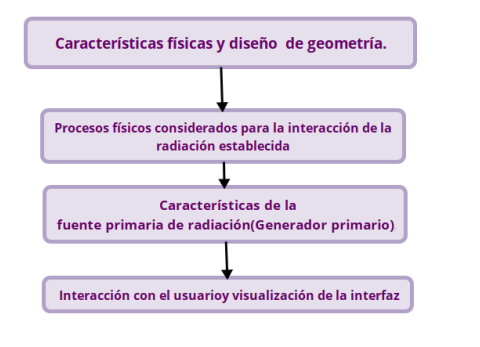
\includegraphics[scale=0.7]{mm}
  \caption{Aspectos importantes dentro
de la simulacion}
  \label{fig:gatos}
\end{figure}



\section{Modelo implementando Geant4}
Esta herramienta hace uso de funciones que permiten el acceso a procesos físicos incorporados en la simulación y a conjuntos de datos,librerías,información de los eventos,entre otros de los que se compone dicho proceso,lo que se constituye como una característica principal de la misma.Dentro del modelo físico y geométrico establecido en la herramienta, se comprende la extensión que permite visualizar;trayectorias de partículas,impactos,geometría,detectores creados y eventos que persisten.Una de estas extensiones, la geometría,permite realizar una descripción detallada de un gran entorno(entorno madre),lo que en este caso es practico en aplicaciones como estas,médicas,donde hacen parte de ese entorno una fuente,detector,paciente o phantom.

Con respecto a los procesos se establece que estos,no dependen del tipo de partícula tratada y tampoco de de los procesos físicos que intervienen en la simulación,dentro de las posibilidades que se pueden dar en  los procesos se tiene:
\begin{itemize}
 \item Generar cambios en las cantidades fisicas.
 \item Generar partículas secundarias.
 \item Suspender, posponer o matar un proceso 
\end{itemize}
y en su seguimiento,los procesos puede actuar en cualquiera de los tres intervalos de espacio-tiempo, ya sea en reposo,a lo largo del step,(mientras transcurre) o en un punto finalizando el proceso,(al final de un step).

Dentro de la lógica de funcionamiento de Geant4 que permite el recrear estos casos,en su núcleo,al momento de realizar el modelamiento de los procesos que  intervienen en la gestión de la simulación,se hace uso de los siguientes elementos:
\begin{itemize}
\item Event:Consiste en la unidad básica de la simulación ejecutada mediante Geant4,la cual comprende la interacción de los primarios y secundarios producidos.
 \item Run:Una recopilación de eventos(event loop), los cuales comparten una descripción física y una geometría en particular.  
 \item Track:Elemento responsable de generar una " pistas o fotografías instantáneas" de aquellas variables físicas asociadas a las partículas que se encuentran procesándose. 
 \item Step:Este elemento guarda información de los cambios que tuvieron las variables físicas en las partículas procesadas. 
\end{itemize}


Los procesos de transporte de partículas en el modelo geométrico son llevados a cabo mediante
la categoría tracking,quien permite la evolución de un estado asociado a un Track proporcionando información en los volúmenes sensibles.

La categoría Track contiene clases para tracks y steps, utilizadas en procesos que se implementan a partir de modelos basados en interacciones físicas.En la categoría de Event se ejecutan los eventos en términos de track y el Run gestiona las colecciones de eventos que comparten un haz y un detector especifico.Por ultimo en la categoría de lectura se acumulan dichos datos para luego ser analizados.




Los elementos anteriormente mencionados se representan mediante las siguientes clases:
\begin{figure}[h]
\centering
  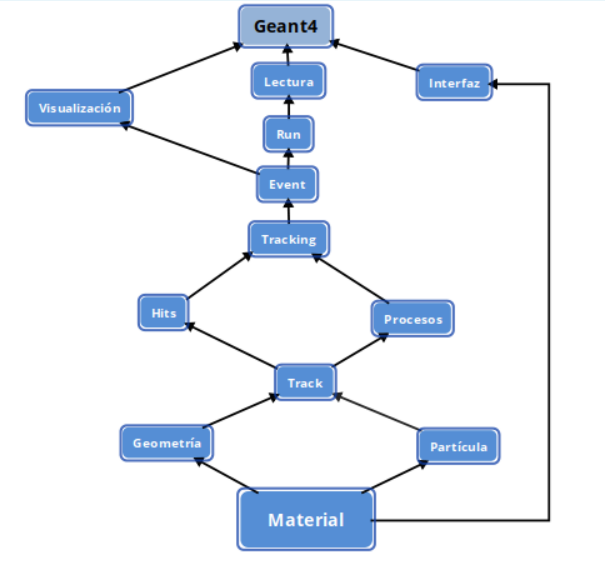
\includegraphics[scale=0.7]{cat}
  \caption{ Diagrama de herramientas en Geant4.}
  \label{fig:gatos}
\end{figure}

\subsection{Procesos incorporados en Geant4.}

Los campos claves presentes en simulaciones donde se establece el paso de partículas a través de la materia son:
 \begin{center}
 \centering
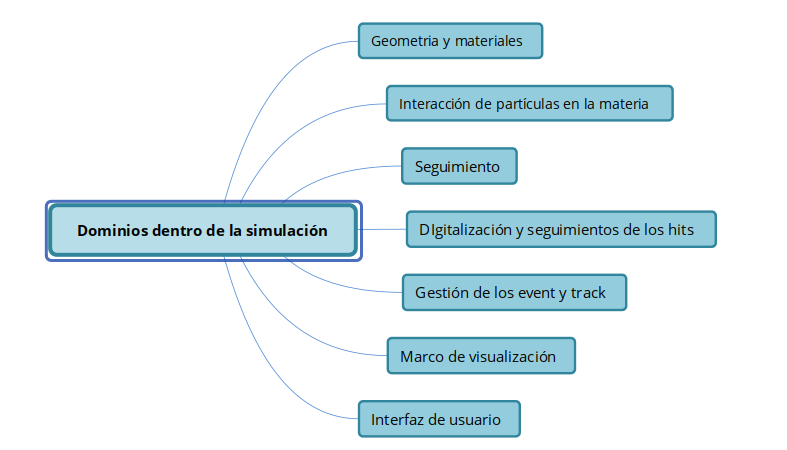
\includegraphics[height=9.0cm]{dom}
\end{center}

Dentro del paquete de herramientas que ofrece Geant4,el usuario esta en capacidad de crear geometrías de materiales  y formas distintas para así definir aquellos elementos "sensitive volume" quienes registran la información "hits" necesaria para una posterior lectura desde el detector.


\begin{itemize}
\item \textbf{Run}: está representada por la clase \textbf{\textit{G4Run}} de la cual se derivan las siguientes:
\subitem \textbf{G4RunManager:}Clase de administrador
\subitem \textbf{G4UserRunAction:} Clase de usuario opcional
\end{itemize}


\begin{itemize}
 \item \textbf {Event}:está representada por la clase \textbf{\textit{G4Event}}  quien tiene como objeto  a la entrada,listar las partículas y a la salida,coleccionar las trayectorias,de la cual se derivan las siguientes clases:
 
 \subitem \textbf{G4EventManager r:}Clase de administrador
\subitem \textbf{G4UserEventAction:} Clase de usuario opcional
\end{itemize}


\begin{itemize}
 \item \textbf {Track}:está representada por la clase \textbf{\textit{G4Track}} de la cual se derivan las siguientes:
 \subitem \textbf{G4TrackingManager:}Clase de administrador
\subitem \textbf{G4UserTrackingAction:} Clase de usuario opcional
\end{itemize}


\begin{itemize}
 \item \textbf {Particle}:está representada por $3$ tipos de clase: \subitem\textbf{G4 Track:} 
\subitem{Posición, información geométrica,entre otros.}
\subitem{Rastreo de partículas}
\subitem \textbf{G4DynamicParticle:}
\subitem{Propiedades dinámicas-físicas de  las partículas,impulso, energía,etc.}
\subitem{Representa una partícula individual.} 
\subitem \textbf{G4ParticleDefinition:}
\subitem{Representa las propiedades estáticas de las partículas}
\subitem
\textbf{G4ProcessManager:}
\subitem{Describe los procesos que comprometen a las partículas}
\subitem{Todos los objetos \textbf {G4DynamicParticle} del mismo tipo de partícula comparten la misma clase}\textbf{G4ParticleDefinition}
\end{itemize}



\begin{itemize}
\item\textbf{Step:} esta representada por la clase \textbf{\textit{G4Step}} de la cual se derivan las siguientes:
\subitem\textbf{G4SteppingManage:} 
Clase de administrador
\subitem\textbf{G4UserSteppingAction:}Clase de usuario opcional.
\subitem{Un punto esta representado por la clases
\textbf{G4StepPoint}}
\end{itemize}




\section {Geometría}
Dentro de este concepto se describe una estructura a partir del manejo autónomo de  figuras geométricas por parte del usuario,esquemas que se acomodan  a las necesidades y objetivos de la simulación,diseño geométrico donde a través de e se propagan partículas eficientemente. 

Para diseñar la geometria inicialmente debe existir un objeto en el cual se   definan las dimensiones del mismo y la forma del volumen teniendo en cuenta la clases para originarlo,en el caso de una esfera la clase asociada seria\textbf{G4Sphere}.Lo que se conoce como \textbf{\textit{Solid Volume}} 


Una vez se haya generado este objeto se establecen los siguientes volumenes: 
\begin{itemize}
 \item Logical Volumen:Quien tiene como función esencial definir el material, el cual es definido a partir de la  clase \textbf{\textit{ G4Material}}. 
 \item Physical Volumen:Define la rotación del volumen original,el numero de copias y la posición respecto al volumen madre.
\item World o volumen madre:Contiene al volumen que se este definiendo siendo este el volumen mas grande entre los mencionados anteriormente.
\end{itemize}



En los procesos físicos que se realizan en Geant4 se describe  la interacción de las partículas con  materiales y/o un volumen determinado.Mediante siete($7$) categorías principales,que son las siguientes:

\begin{itemize}
 \item Electromagnetic
\item  Hadronic
\item  Photolepton-hadron
\item  Decay
\item  Optical
\item  Transportation
\item  Parameterization
 \end{itemize}

 Procesos,modelos,categorías que el usuario puede elegir a conveniencia según el tipo de partícula.  

\section{Procesos Físicos}

Dentro de la física electromagnética planteada en Geant4 se manejan las  interacciones de tipo electromagnético de partículas como:Fotones,leptones, hadrones e iones.

\begin{itemize}
 \item Conjunto de categorías de clase relacionadas al paquete electromagnético.  
\end{itemize}

\begin{figure}[h]
\centering
  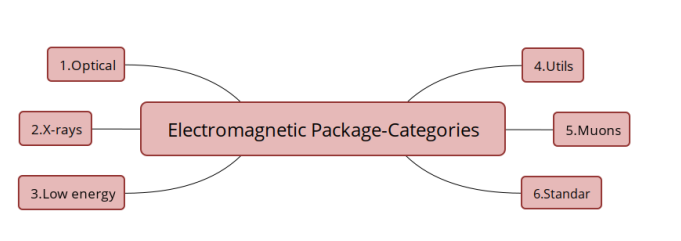
\includegraphics[scale=0.7]{packa}
  \end{figure}
  
\begin{itemize}
\item$1.$ Establece un código determinado para fotones ópticos
\item$2.$Se establece un código especifico con respecto a la
física de rayos X.
\item$3.$Proporciona modelos alternativos a energías mas bajas con respecto a las tratadas en la categoría estándar
\item$4.$Grupo de clases usadas por las otras categorías.
\item$5.$ Interacciones con muones.
\item$6.$ Manejo de procesos básicos para las interacciones de  positrones,electrones y fotones y hadrones.
\end{itemize}
  

\section{Manejo de la información (Adquisición e implementación de datos).}



% 
% 
% 
% \subsection{Motivación}\index{Motivación}
% 
% Los modelos Logit se comportan como una herramienta científica avanzada, genera instrumentos y procedimientos que permitirán validar, mejorar y actualizar los procesos estadísticos.
% \\\\
% Los modelos de elección cualitativa son muy útiles y muy utilizados en la economía, porque muchas decisiones pueden ser tomadas a partir de simples respuestas como un sí o un no, podemos mencionar por ejemplo la decisión de una empresa si va decidir retribuir servicio de sus utilidades a sus accionistas o no, votar por un político o no, si un individuo viene a trabajar o no. Estos son distintos casos de los modelos tradicionales. El objetivo de los modelos de elección cualitativa es encontrar la probabilidad de que algo ocurra; por ello los modelos de elección cualitativa son también conocidos como modelos de probabilidad.
% \\\\
% 
% \subsection{Descripción Teórica del Modelo}\index{Descripción Teórica del Modelo}
% 
% Los modelos Logit son de respuesta binaria (0 y 1) se usan como un instrumento recomendable para calcular la probabilidad de respuesta, indicando la construcción y forma del modelo y el análisis de algunos estadísticos requeridos.
% \\\\
% La modelización Logit es similar a la regresión tradicional salvo que utiliza como función de estimación a la función logística en lugar de utilizar a la lineal. Con la modelización Logit, el resultado del modelo es la estimación de la probabilidad de que un nuevo individuo pertenezca a un grupo o a otro (probabilidad de éxito o fracaso, si o no, etc.). Además, al tratarse de un análisis de regresión, también es posible identificar las variables más importantes que explican las diferencias entre grupos.
% \begin{align} 
% \begin{split}
% P(y=1/x) = P(y=1/x_{1},x_{2},...,x_{k})
% \end{split}					
% \end{align}
% 
% donde x denota el conjunto total de variables explicativas. En el MPL, se supone que la probabilidad de respuesta es lineal en un conjunto de parámetros $\beta _{k}$. Para evitar las limitaciones del MPL, considere una clase de modelos de respuesta binaria de la forma:
% \begin{align} 
% \begin{split}
% P(y=1/x)=F(\beta _{0}+\beta _{1}x_{1}+\beta _{2}x_{2}+...+\beta _{k}x_{k})=F(\boldsymbol{x\beta})
% \end{split}					
% \end{align}
% 
% donde F es una función que asume valores estrictamente entre cero y uno, para todos los números reales z. Esto asegura que las probabilidades de respuesta estimada están estrictamente entre cero y uno. La función F, entre las muchas sugeridas, es la función logística, cuya representación es:
% \begin{align} 
% \begin{split}
% F(x\beta)=\Lambda(z)=\frac{e^{x\beta}}{1+e^{x\beta}}
% \end{split}					
% \end{align}
% 
% que está entre cero y uno para todos los números reales z. Esta es la función de distribución acumulada (fda) para una variable aleatoria logística estándar. La función logística es creciente, y aumenta con más rapidez en z = 0. El comportamiento de la función es el siguiente: F(z) $\rightarrow $ 0 a medida que z $\rightarrow -\infty $ , y F(z)$\rightarrow $1 a medida que z$\rightarrow \infty$. (Ver gráfica en \textbf{Anexo1}).
% 
% \subsection{Definición Matemática}\index{Definición Matemática}
% 
% El modelo Logit puede derivarse a partir de un modelo de variable latente subyacente. Sea y* una variable inobservable, o latente, determinada por:
% \begin{align} 
% \begin{split}
% y^{*}=\beta_{0}+x\beta+e,y=1[y^{*}>0]
% \end{split}					
% \end{align}
% 
% donde se introduce la notación 1[.] para definir un resultado binario. La función 1[.] recibe el nombre de función de indicador, que asume el valor de uno si el evento dentro de los corchetes es verdadero y de cero si no lo es. Por tanto, y es uno si y* $>$ 0 y y es cero si y* $\leq$ 0.
% \\\\
% Bajo el supuesto que ``x'' es independiente de ``e'' y que este último tiene la distribución logística estándar, ``e'' se distribuye simétricamente en torno a cero, lo cual significa que 1 - F(-z) = F(z) para todos los números reales z. A partir de (3.4) y de los supuestos establecidos al inicio del párrafo, es posible calcular la probabilidad de respuesta para y:
% 
% \begin{align} 
% \begin{split}
% P(y=1/x)   &=P(y*>0/x)=P[x\beta+e>0/x]=P[e>-(\beta_{0}+x\beta)/x]\\
% &=1-F[-(\beta_{0}+x\beta)]=F(\beta_{0}+x\beta)
% \end{split}					
% \end{align}
% 
% \subsection{Impacto marginal}\index{Impacto marginal}
% 
% Como en todo modelo de estimación,  el objetivo principal del modelo Logit es explicar los efectos de las $x_{j}$ sobre la probabilidad de respuesta P(y =1/x). La formulación de la variable latente tiende a dar la impresión de que lo que principalmente interesa son los  efectos de cada $x_{j}$ sobre y*. Pero la variable latente y* rara vez tiene una unidad de medición bien definida. (Por ejemplo, y* puede ser la diferencia en niveles de utilidad de dos acciones diferentes.) Por tanto, las magnitudes de cada $\beta _{k}$ no son, por sí mismas, especialmente útiles en contraste con el modelo de probabilidad lineal.
% \\\\
% Para la mayoría de los propósitos, se quiere estimar el efecto de $x_{j}$ sobre la probabilidad de éxito P(y =1/x), pero esto se complica por la naturaleza no lineal de la función logística. 
% Para hallar el efecto parcial de las variables aproximadamente continuas sobre la probabilidad de respuesta, es necesario recurrir al cálculo. Si $x_{j}$ es una variable aproximadamente continua, su efecto parcial sobre p(x) = P(y = 1/x) se obtiene de la derivada parcial:
% 
% \begin{align} 
% \begin{split}
% \frac{\partial p(x)}{\partial x_{j}}=\frac{\partial F(x\beta)}{\partial x}=\frac{\partial F(x\beta)}{\partial x\beta}\frac{\partial x\beta}{\partial \beta}=f(\overline{x}\beta)\beta _{j}
% \end{split}					
% \end{align}
% 
% Ahora, si por ejemplo, $x_{j}$ es una variable explicativa binaria discreta, entonces el efecto parcial de cambiar $x_{j}$ de cero a uno, manteniendo todas las demás variables fijas, simplemente es:
% \begin{align} 
% \begin{split}
% \frac{\Delta P(y=1/x) }{\Delta x_{j}}   &=P(y=1/x_{j}=1)-P(y=1/x_{j}=0)\\
% &=F(\beta _{0}+\beta _{1}x_{1}+...+\beta _{k}x_{k}/x_{j}=1)-F(\beta _{0}+\beta _{1}x_{1}+...+\beta _{k}x_{k}/x_{j}=0)
% \end{split}					
% \end{align}
% 
% \section{Modelo Probit}\index{Modelo Probit}
% 
% Los Modelo Probit son aquellos que pertenecen a la clase de modelos de respuesta binaria, es decir, la variable dependiente es una variable dicotómica, donde toma 1 para indicar el éxito en la variable de análisis y 0 en el caso de no ser así.
% \\
% Por ejemplo se asume una variable observada (latente) que debe traspasar un umbral para que la variable dependiente tome el valor de 1,la estimación d estos modelos no puede ser realizada por MCO (Mínimos cuadrados ordinarios)ya que la variable dependiente es inobservable por lo que se recurre al uso de Máxima Verosimilitud haciendo supuestos sobre la distribución de los errores.Cuando los errores se consideran distribuidos de manera normal, entones se obtiene un Modelo Probit .
% \\
% Con esta especificación,la variable dependiente dicotómica tiene la probabilidad de 2 opciones Pr(y=1/x) o la Pr (y=0/x) que dependen de los valores que toman las variables de control especificadas como las variables sociodemográficas, socioeconómicas representadas mediante una combinación lineal ($x_{i}\beta$).El modelo se especifica de la siguiente forma :
% 
% \begin{align} 
% \begin{split}
% P(y=1/x)= Pr(y^{*}>0)=F(x\beta)
% \end{split}					
% \end{align}
% 
% 
% Si definimos el modelo de la siguiente manera:
% \begin{align} 
% \begin{split}
% P(y=1/x)=G(\beta_{0}+x_{1}\beta_{1}+ ... + x_{K}\beta_{K})=G(\beta_{0}+x\beta)
% \end{split}					
% \end{align}
%  
% 
% donde G es una funcion que adopta valores entre cero y uno para todos los numeros reales Z,donde G representa la funcion de distribucion acumulativa.
% 
% Debido a que el modelo Probit es un modelo de vaiable dependiente limitada,la estimacion de parametros se hace por el metodo de Maxima Verosimilitud.Este modelo sugiere que se elijan como estimados los valores de los parametros que maximizen el logaritmo de la funcion de verosimilitud.
% La funcion logaritmica de verosimilitud para la observacion i se define como: 
% 
% \begin{align} 
% \begin{split}
% \lambda(\beta)= yi log(G(Xi\beta)) + (1-yi)log(1-G(Xi\beta))
% \end{split}					
% \end{align}
% 
% El logaritmo de la funcion de verosimilitud para una muestra de tamano n se define como:  
% 
% \begin{align} 
% \begin{split}
% L= \sum_{i=1}^{n} \lambda(\beta)
% \end{split}					
% \end{align}
% 
% El estimador de maxima verosimilitud de $\beta$,denotado por $\beta$  que maximize el logaritmo de verosimilitud.Las propiedades de los estimadores de maxima verosimiltud del modelo son conistentes,asintoticamente normales y asintoticamente eficientes.
% \\
% Ahora conociendo los efectos de los cambios en las variables explicativas sobre las probabilidades de que cualquier observaion perteneza a uno de los 2 grupos (y=0,y=1) se emplea una derivada parial definida como:
% 
% \begin{align} 
% \begin{split}
% \frac{\partial x }{\partial xj} = g(\beta 0 +X\beta )\beta
% \end{split}					
% \end{align}
% 
% 
% El termino g(z) corresponde a una funcion de densidad de probabilidad.Dado que en el modelo Probit G(.) es una funcion de distribucion acumulativa estrictamente positiva,g(z)>0 para toda Z,el signo del efecto parcial es el mismo que el de $\beta$.
% 
% 
% Ahora para probar la significania de cada uno de los coeficientes estimados se lleva a cabo la prueba hipotesis Ho :$\beta$=0,con un t estadistico.Para probar la significancia de variables conjuntamente existen diferentes estadisticos como el estadistico Wald y el estadistico de la razon de verosimilitud entre otros. En estos 2 casos se emplea una distribucion chi cuadrado.
% 
% Mediante un caso practico analizaremos ambos modelos e interpretaremos los resultados
% Estimamos en Stata el siguiente modelo para la probabilidad de estar
% desempleado en Colombia en función de la edad, el genero, la situacion marital, la educacion, el ingreso no laboral y la localizacion geografica.
% \\\\
% . probit desocupado edad mujer soltero educ jefe inla caba 
% Ver resultados en \textbf{Anexo2}.
% \\\\
% A diferencia de los modelos de Mínimos Cuadrados Ordinarios (MCO), estos modelos tienen que ser interpretados cuidadosamente.Empezando que los valores de estos coeficientes no tienen una interpretación cuantitativa (solo es interpretable el signo de los mismos).A la vez analizaremos los efectos marginales de cada variable para realizar una interpretación cuantitativa del efecto de cada variable sobre la probabilidad de estar desocupado.
% \\\\
% Interpretando cuantitativamente cada uno de los efectos
% marginales.Las variables explicativas que son continuas:
% \\\\
% .La interpretación del valor -0.0020344, que corresponde al efecto marginal de la variable años de educación (educ) donde para una persona con las características consideradas un aumento en un año de
% educación provoca un cambio en la probabilidad predicha de -0.0020344, es decir, las 2 probabilidades de estar desocupado se reduciría en 0.203 puntos porcentuales (-0.0020344*100),dado todo lo demás constante.
% .La interpretación para el efecto marginal de la variable edad es equivalente. Para una persona con las características consideradas, un aumento en un año de edad reduce la probabilidad
% predicha de estar desempleado en 0.022 puntos porcentuales (-0.0002215*100), ceteris paribus.
% \\\\
% Para el caso del efecto marginal de las variables dummies (como mujer, soltero, jefe y caba) recuerden que se computan de diferente manera pero se interpreta de manera equivalente.
% 
% • El hecho de ser jefe de hogar, para un hombre casado que es jefe de familia, con 17 años de educación, edad e ingreso no laboral promedio y que resida en la CABA, reduce su probabilidad predicha de estar desempleada en 1.87 puntos porcentuales (-0.0187869*100).
% • De la misma forma, el hecho de residir en CABA, dado todo lo demás, reduce su probabilidad predicha de estar desempleada en 0.19 puntos porcentuales (-.0019124*100).
% \\\\
% Como notarán, se ha hecho énfasis en aclarar que en el caso de los modelos de elección binaria si se multiplica por 100 al efecto marginal, se está midiendo el efecto del cambio en una unidad de X sobre la probabilidad predicha. Ese cambio es en puntos porcentuales y no en tanto por ciento.En el primer caso se usa para indicar un cambio marginal, mientras que el segundo se aplica cuando se trata
% de cambios proporcionales.
% Por ejemplo, según se muestra en la segunda salida de Stata, la probabilidad de desempleo para un hombre casado que es jefe de familia, con 17 años de educación, edad e ingreso no laboral promedio y que resida en la CABA es de 0.02056653 (es decir, 2 por ciento de probabilidad). Dijimos que el efecto marginal de la educación (educ) para este caso es de 0.20 puntos porcentuales, es decir si en
% lugar de tener 17 años de educación tuviera 18 (1 año más) entonces la probabilidad pasaría a ser 1.8\% (es decir, el 2 por ciento original menos 0.20 puntos porcentuales).
% La forma incorrecta de interpretar los modelos probit y logit es si habláramos del cambio de probabilidad como una reducción del 0.02\% (cambio proporcional), porque en ese caso se entiende que
% la probabilidad predicha para ese caso seria 1.9996 por ciento,es decir hacer 2*(1-0.0002),lo cual es incorrecto. 
% 
% 
% 
% 
% \section{Problema Aplicativo}\index{Problema Aplicativo}
% 
% La entidad financiera ABC, destina \$800,000,000 de su capital a otorgar créditos personales de acuerdo a las siguientes convenciones:
% 
% -El Supervisor bancario, establece una tasa de severidad (LGD) de 45\% para el banco, ya que este no cuenta con un modelo interno para la estimación de dicho parámetro.
% 
% -El Supervisor, establece las categorías crediticias basándose en la probabilidad de incumplimiento (PD), de la siguiente manera:
% Cliente normal(0 – 20\%), cliente con problemas potenciales(20\%-40\%), cliente deficiente(40\%-60\%), cliente dudoso(60\%-80\%) y pérdida: (80\%-100\%)
% 
% -Basándose en los lineamientos de riesgo que sigue el banco, se establece que los préstamos personales en mención se harán de la siguiente manera:
% Clientes normales: 35\%, cliente con problemas potenciales: 30\%, cliente deficiente: 20\%, cliente dudoso: 10\% y pérdida: 5\% del capital invertido en préstamos.
% 
% -Se pide al banco declarar el gasto en provisiones que hará, teniendo en cuenta que para su cálculo sigue una metodología de Pérdidas Esperadas.
% \\\\
% 
% \textbf{Desarrollo}
% 
% \subsection{Estimación con el Modelo Logit}\index{Estimación con el Modelo Logit}
% 
% Lo primero que se realizó fue realizar una estimación mediante el modelo Logit. Se regresionó la variable dependiente ``default'' (variable dicotómica discreta que toma el valor de 1 si el individuo cayó en default, y 0 en caso contrario) con respecto a las variables explicativas edad, rcuota\_ingreso, ingreso, nro\_ctas, nro\_default\_anterior, nro\_prest\_hipotec y nro\_depend. Como resultado de la estimación, obtuvimos que todos los parámetros eran significativos excepto el coeficiente de la variable nro\_prest\_hipotec (Ver en \textbf{Anexo3}).
% \\\\
% Para comprobar que dicha variable no era significativa, aplicamos el test de Wald, el test nos permite asegurar que dicha variable no era significativa. Por tanto, regresioanamos nuevamente el modelo logit, pero esta vez sin la variable en cuetión. El resultado obtenido es que ahora todas las variables consideradas son significativas. (Ver \textbf{Anexo4} y \textbf{Anexo5})
% 
% \subsection{Estimación con el Modelo Probit}\index{Estimación con el Modelo Probit}
% Análogamente al caso anterior, realizamos una regresión mediante el modelo Probit de la variable cualitativa discreta dcicotómica ``default'' con respecto a todas las variables exógenas encontradas en la base de datos ``data\_pd''. De la misma manera que con el modelo Logit, los resultados arrojan que la variable independiente nro\_prest\_hipotec es la única que no es significativa, al estimar nuevamente el modelo sin considerar esta vez dicha variable, se obtiene un modelo con todas las variables significativas. (Ver \textbf{Anexo6} y \textbf{Anexo7}) 
% 
% \subsection{Comparando entre Modelos}\index{Comparando entre Modelos}
% Una vez que hemos realizado las estimaciones con los modelos Logit y Probit, el siguiente paso es elegir entre estos dos modelos, el criterio de elección es: elegir el modelo que tenga mayor capacidad de predicción acetdad, esto será posible analizando la Potencia recurriendo al comando ``lstat''. Los resultados del test indican que con el modelo Logit se acierta en el 67.45\% de los casos, mientras que el modelo Probit acierta en el 67.44\%. (Ver \textbf{Anexo8} y \textbf{Anexo9})  
% \\
% Al contrastar ambos resultados, se aprecia que el modelo logit es ligeramente mejor que el modelo Probit, debido a que la diferencia obtenida del test entre ambos modelos es mínima; se podría decir, en este caso particular que es indistinto optar por cualquiera de ellos. Sin embargo, el modelo elegido para desarrollar los pasos siguientes es el Modelo Logit.
% \\\\
% Finalmente para validar nuestro modelo obtenido, analizamos la Curva ROC mediante el comando ``lroc'', el resultado muestra que el área es 0.7436, valor superior a 0.5. Por lo tanto, es correcto decir que nuestro modelo de elección discreta dicotómica: Logit, está bien especificado. (Ver \textbf{Anexo10}).
% 
% \subsection{Probabilidad de Default}\index{Probabilidad de Default}
% 
% Ya que contamos con el modelo adecuado, además que está validado, lo que realizaremos ahora es estimar las probabilidades de default. Lo primero a hacer es obtener la probabuilidad de default para cada individuo. Es decir, obtendremos la probabilidad que cada individuo con sus características específicas cumpla sus pagos.
% \\
% Después de esto, se ordena dichas probabilidades de menor a mayor, para poder facilitar la agrupación, ya que se categorizará a las personas en 5 niveles de riesgo, de acuerdo al nivel de probabilidas obtenida, dicha categorización será de la siguiente manera:
% 
% \begin{table}[H]
% \caption{Ranking Crediticio}
% \centering
% \begin{tabular}{llr}
% \toprule
% \multicolumn{2}{c}{Categorías} \\
% \cmidrule(r){1-2}
% Cliente & PD(\%) \\
% \midrule
% Normal & $[0 - 20]$ \\
% CPP & $[20 - 40]$ \\
% Deficiente & $[40 - 60]$ \\
% Dudoso & $[60- 80]$ \\
% Pérdida & $[80 - 100]$ \\
% \bottomrule
% \end{tabular}
% \end{table}
% 
% Una vez categorizado a cada individuo, se debe calcular la probabilidad default promedio de cada categoría. Dichos valores representan el valor esperado de la PD por cada categoría. Los resultados de esta operación se meustran en el \textbf{Anexo11}.
% \\\\
% Estos resultados nos permite corroborar con la teoría, ya que se aprecia que la esperanza que los individuos normales caigan caigan en default es baja (17.08\%), mientras la esperanza que los individuos categorizados en pérdida caigan en defaul es muy alta (92.07\%)
% 
% \subsection{Pérdida Esperada}\index{Pérdida Esperada}
% 
% Contamos ya con el promedio de la probabilidad de incumplimiento de cada categoría crediticia que se ha calculado anteriormente, con la tasa de severidad (LGD) de 45\% establecido por el Supervisor bancario (SBS para el caso peruano) y el saldo expuesto determinado por la entidad financiera ABC de la siguiente manera: 
% \begin{table}[H]
% \caption{Saldo Expuesto}
% \centering
% \begin{tabular}{|l|l|r|}
% \toprule
% \multicolumn{2}{c}{Categorías} \\
% \cmidrule(r){1-2}
% Cliente & \ \ Porcentaje del\\ & capital invetido \\
% \midrule
% Normal & \ \ \ \ \ \ \ \ \ \ \ \ $35\%$ \\\hline
% CPP & \ \ \ \ \ \ \ \ \ \ \ \ $30\%$ \\
% Deficiente & \ \ \ \ \ \ \ \ \ \ \ \ $20\%$ \\
% Dudoso &  \ \ \ \ \ \ \ \ \ \ \ \ $10\%$ \\
% Pérdida &  \ \ \ \ \ \ \ \ \ \ \ \ $5\%$ \\
% \bottomrule
% \end{tabular}
% \end{table}
% Ahora, a partir de estos 3 datos es posible hallar la pérdida esperada para dicha entidad.(Ver \textbf{Anexo12})
% \\
% Los resultados nos dicen que el banco deberá tener una mayor cantidad de  provisiones para las categorías de clientes que se encuentren  con problemas potenciales y/o sean deficientes; aunque sus probabilidad de incumplimiento no sean las más  altas, la causa se debe a que tienen un mayor porcentaje del capital invertido.
% \\\\
% Los clientes normales y dudosos presentan una menor perdida esperada, pero  no son la categoría que necesitan menos provisiones. En el caso de clientes normales aunque tengan una baja probabilidad de incumplimiento, pero presentan un alto porcentaje del capital invertido (el más alto entre las cinco categorías). Para los clientes dudosos, es la situación contraria;  presentan una alta probabilidad de incumplimiento y por lo tal el capital invertido no es tan alto.
% \\\\
% Y con menor cantidad de provisiones se encuentra los clientes que son categorizados como pérdida ya que cuentan con una alta probabilidad de incumplimiento; justamente se espera que  la perdida esperada no sea tan alta, y para esto el banco asigna un menor porcentaje de su capital.\\
% En suma la perdida esperada total es \$132,404,686.20; por lo tal el banco tendrá que declarar el gasto en provisiones igual a ese mismo monto.\\
% 
% %%%%____________mio
% 
% 
% -----------------------------
% \chapterimage{lab} % Chapter heading image
% 
% \chapter{Simulación electromagnética con Geant4 }
% %pag78 MONTE CARLO
% \section{Introducción}\index{Introducción}
% Contar las variables indica cuántas veces ha ocurrido un evento. Mientras que el uso de la regresión modelos de conteo es relativamente reciente, incluso una breve encuesta de aplicaciones recientes ilustra cómo estos resultados son comunes y la importancia de este tipo de modelos. Los ejemplos incluyen el número de pacientes, hospitalizaciones, homicidios diarios, conflictos internacionales, bebidas consumidas, accidentes de trabajo, nuevas empresas, y las detenciones por la policía, por nombrar sólo algunos.
% \\\\
% Mientras que el modelo de regresión lineal a menudo se ha aplicado para contar los resultados, esto puede resultar en que las estimaciones sean ineficientes, inconsistentes y sesgadas. A pesar de que hay situaciones en las que el la regresión lineal  proporciona resultados razonables, es mucho más seguro de usar modelos diseñados específicamente para el conteo de resultados. En este capítulo   se estudiara el modelo de  regresión de Poisson (PRM).
% \\
% 
% %%%%%%%%%%_________-mio
% \textbf{Problema Aplicativo}
% \begin{itemize}
% 
%  \item z
% \end{itemize}
% 
% \section{Distribución de Poisson}\index{Distribución de Poisson}
% 
% La distribución de Poisson univariado es fundamental para la comprensión de los modelos de conteo. En consecuencia, comenzamos explorando esta distribución. Sea y una variable aleatoria que indica la número de veces que se ha producido un evento. Si Y tiene una distribución de Poisson, a continuación:
% 
% \begin{equation}
% Pr(y | \mu ) =\frac{{e}^{\mu }\mu^{y }}{y!}
% \end{equation}
% 
% donde  $\mu> 0 $• es el único pa
% \section{Objetivo General}\index{Objetivo General}rámetro que define la distribución. La manera más fácil de conseguir un sentido de esta distribución es comparar la trama de la probabilidad pronosticada para diferentes valores de la tasa parámetro $\mu$ (etiquetado como mu en el gráfico):
% 
% \begin{center}
% 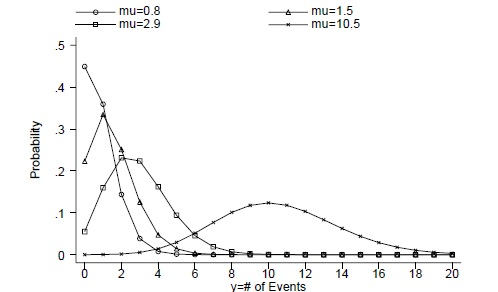
\includegraphics[height=6cm]{1}
% \end{center}
% 
% La trama muestra cuatro características de la distribución de Poisson que son importantes para la comprensión modelos de regresión para el recuento:
% \begin{itemize}
% \item  $\mu$ es la media de la distribución. Como  $\mu$  aumenta, la masa de la distribución se desplaza hacia la derecha.
%  \item $\mu$ es también la varianza. Por lo tanto, $Var (y) = \mu$, que se conoce como equidispersión. En los datos reales, muchas variables de recuento tienen una varianza mayor que la media, que se llama sobredispersión.
%  \item Como $\mu$ aumenta, la probabilidad de que un cero disminución de los recuentos. Para muchas variables de recuento, hay ceros que las predichas por la distribución de Poisson más observado.
%  \item Como $\mu$ aumenta, la distribución de Poisson se aproxima a una distribución normal. Esto se muestra por la distribución de $\mu = 10,5$.
%  \end{itemize}
% 
% \section{Modelo de Regresión de Poisson}\index{Modelo de Regresión de Poisson}
% 
% El modelo de regresión de Poisson (PRM) se extiende de la distribución de Poisson al permitir que cada observación tener un valor diferente de $\mu$. Más formalmente, el PRM asume que el recuento observado para la observación i se extrae de una distribución de Poisson con $\mu_{i}$ de media, donde $\mu_{i}$  se estima a partir  de las características observadas. Esto se refiere a veces como la incorporación de heterogeneidad observada, y conduce a la ecuación estructural:
% \\
% \begin{equation}
% \mu_{i}  =E(y_{i}|x_{i})=exp(x_{i}\beta )
% \end{equation}
% 
% Por lo tanto la distribución de Possion con la variables explicativas x, seria:
% \begin{equation}
% Pr(y | x) =\frac{{e}^{\mu_{i} }\mu_{i}^{y }}{y!}
% \end{equation}
% Tomando el exponencial de  $x\beta$ para  $\mu$ debe ser positivo, lo cual  necesario ya que el conteo sólo puede ser 0 o positivo. Para ver cómo funciona esto, considere el modelo de regresión de Poisson con una sola variable independiente $\mu$ =exp ($\alpha$ $+$ $\beta x$), que puede ser trazada como:
% 
% \begin{center}
% 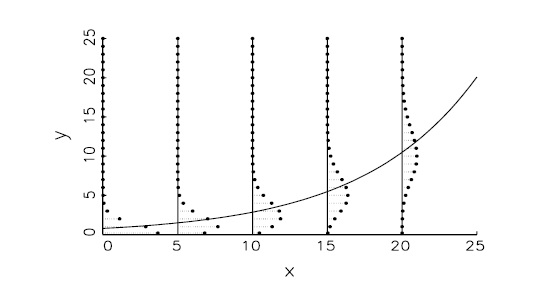
\includegraphics[height=6cm]{2}
% \end{center}
% 
% En este gráfico, la media  $\mu$, que se muestra por la línea curva, aumenta a medida que aumenta x. Para cada valor de  $\mu$, la distribución alrededor de la media se muestra por los puntos y que representan la probabilidad de cada conteo. Interpretación del modelo implica evaluar cómo los cambios en las variables independientes afectan a la media condicional y las probabilidades de varios conteos.
% 
% \subsection{Estimación por máxima verosimilitud }
% \begin{equation}
% lnt =\sum_{i=1}^{n}({-\mu+yln\mu-ln(y!)})
% \end{equation}
% \begin{equation}
% lnt=\sum_{i=1}^{n}({-e^{x\beta}+yx\beta-ln(y!)})
% \end{equation}
% 
% Derivamos la ecuación respecto de $\beta$
% \begin{equation}
% \frac{\partial lnt }{\partial \beta}=\sum_{i=1}^{n}({-xe^{x\beta}+yx})=0
% \end{equation}
% \begin{equation}
% \sum_{i=1}^{n}({xe^{x\beta}})=\sum_{i=1}^{n}{(y_{i}x_{i}})
% \end{equation}
% 
% \begin{equation}
% \frac{\partial^2 lnt }{\partial \beta^2}= -\sum_{i=1}^{n}({xxe^{x\beta}})
% \end{equation}
% 
% \section{Ejemplo de una estimación del modelo de regresión de Poisson en Stata}\index{Ejemplo de una estimación del modelo de regresión de Poisson en Stata}
% 
% Para este ejemplo, utilizamos datos de Long (1990) sobre el número de publicaciones producido por Ph.D. bioquímicos. Las variables consideradas son\\
% . use couart2, clear\\
% . describe\\
% 
% \begin{center}
% \includegraphics[height=4.5cm]{3}
% \end{center}
% 
% . summarize\\
% 
% \begin{center}
% 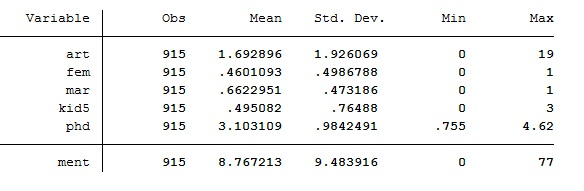
\includegraphics[height=5cm]{4}
% \end{center}
% 
% Las diferencias entre los científicos en sus índices de productividad podría deberse a factores como el género, el estado civil, el número de jóvenes niños, el prestigio del programa de postgrado, y el número de artículos escritos por el mentor de un científico. Para dar cuenta de estas diferencias, añadimos estas variables como variables independientes, donde la variable dependiente sera el numero de artículos en los  últimos 3 años de doctorado.
% \\\\
% Ahora utilizaremos el siguiente comando para estimar el modelo.\\
% . poisson art fem mar kid5 phd ment, nolog\\
% 
% \begin{center}
% 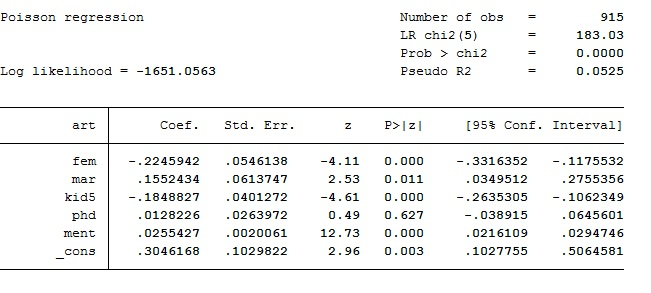
\includegraphics[height=6cm]{5}
% \end{center}
% 
% La manera  en la cual se interpreta  un modelo de conteo depende si se está interesado en el valor esperado de la variable de recuento o en la distribución de los recuentos. Si el interés está en el recuento esperado, varios métodos se pueden utilizar para calcular el cambio en la expectativa de un cambio en una independiente variable.
% \\
% Si el interés está en la distribución de los recuentos o tal vez sólo la probabilidad de que un recuento específico, la probabilidad de que un recuento para un nivel dado de las variables independientes se puede calcular.
% \begin{itemize}
%  \item Factor de Cambio en la E (y / x)\\
% Quizás el método más común de interpretación es el factor de cambio en la tarifa. Si definimos
% E (y / x,$ x_{k}$) como el recuento esperado para un determinado x donde notamos explícitamente el valor de $x_{k}$, y definir E (y / x, $x_{k}$ + $\delta$) como el recuento de espera después de aumentar$ x_{k}$ por unidades $\delta$, entonces
% \begin{equation}
% \frac{E (y / x, x_{k}+ \delta)}{E (y / x, x_{k})}=e^{\beta_{k}\delta}
% \end{equation}
% Por lo tanto, los parámetros pueden ser interpretados como
% Para un cambio de $\delta$ en $x_{k}$, el recuento esperados aumenta en un factor de $exp(\beta_{k}\delta)$, teniendo a  todas las otras variables constantes.
%  \item Cambio porcentual en el E (y / x)\\
% Por otra parte, el porcentaje de cambio en el recuento esperado para un cambio unitario $\delta$ en  $x_{k}$, la celebración de otra las variables constantes, se puede calcular como:
% 
% \begin{equation}
% 100*\frac{E (y / x, x_{k}+ \delta)-E (y / x, x_{k})}{E (y / x, x_{k})}= 100*[exp (\beta_{k}*\delta) - 1]
% \end{equation}
% \end{itemize}
% \subsubsection{Calculamos el factor y el cambio en el E (y / x)}
% Coeficientes de cambio Factor se pueden calcular utilizando listcoef:\\
% . poisson art fem mar kid5 phd ment, nolog\\
% . listcoef fem ment, help\\
% 
% \begin{center}
% 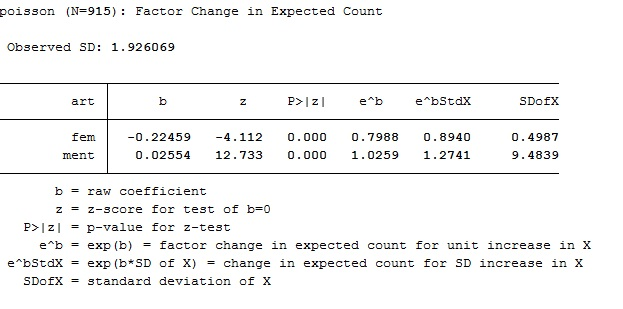
\includegraphics[height=6cm]{6}
% \end{center}
% 
% Por ejemplo, los coeficientes de fem y ment pueden ser interpretados como: Ser una científica disminuye el número esperado de artículos por un factor de 0.80, manteniendo  las demás variables constantes.
% \\
% Para un aumento de una desviación estándar de la productividad del mentor, aproximadamente 9,5 artículos, un medias aumento de la productividad del científico por un factor de 1,27, manteniendo constante otras variables.Para calcular el porcentaje de cambio utilizamos el comando:
% 
% listcoef fem ment, percent help\\
% 
% \begin{center}
% 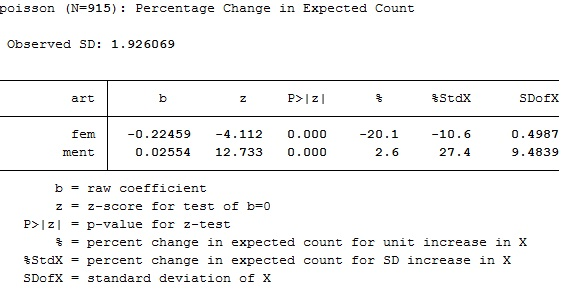
\includegraphics[height=6cm]{7}
% \end{center}
% 
% Por ejemplo, los coeficientes de variación porcentual de fem y ment pueden ser interpretados como:\\
% Ser una científica disminuye el número esperado de artículos en un 20 por ciento, manteniendo todas las otras variables constantes. Por cada artículo adicional por parte del mentor, predijo de un científico de la productividad media aumenta en un 2,6 por ciento, manteniendo constantes otras variables.
% \subsubsection{Cambio marginal en E (y / x)}
% Otro método de interpretación es el cambio marginal en  E (y / x)
% \begin{equation}
% \frac{\partial E (y /  x_{k})}{\partial  x}=E (y / x)\beta_{k}
% \end{equation}
% Para $\beta_{k}> 0$ es  mayor  el valor actual de E (y | x), mayor es la tasa de cambio; para $\beta_{k} <0$,es menor es la tasa de cambio. El marginal respecto de $x_{k}$ depende tanto $\beta_{k}$ y E (y/ x).
% Por lo tanto, el valor de la marginal depende de los niveles de todas las variables en el modelo. En la práctica, este medida a menudo se calcula con todas las variables se encuentren en su medio.
% \subsubsection {Ejemplo de cambio marginal utilizando mfx compute}
% Por default, mfx compute calcula el cambio marginal con variables se encuentren en su medio:\\
% . mfx compute\\
% 
% \subsection{Interpretación utilizando probabilidades predichas}
% Los parámetros estimados se pueden utilizar también para calcular probabilidades predichas utilizando la siguiente fórmula:
% \begin{equation}
% \widehat{Pr}(y =m| x) =\frac{{e}^{-x \widehat{\beta}}({{x \widehat{\beta}}})^{m }}{m!}
% \end{equation}
% Probabilidades pronosticadas en los valores especificados se pueden calcular utilizando prvalue. Las predicciones de los valores observados  para todas las observaciones se pueden calcular usando prcounts.\\
% . poisson art fem mar kid5 phd ment, nolog\\
% . prcounts prm, plot max(9)\\
% . d prm*\\
% 
% 
% 
% %----------------------------------------------------------------------------------------
% %	PART
% %----------------------------------------------------------------------------------------
% 
% \part{Parte Dos}
% 
% %----------------------------------------------------------------------------------------
% %	CHAPTER 3
% %----------------------------------------------------------------------------------------
% \chapterimage{Ap} % Chapter heading image
% 
% \chapter{Laboratorio Virtual}
% 
% \section{Introducción}\index{Introducción}
% Para esto 
% Contar las variables indica cuántas veces ha ocurrido un evento. Mientras que el uso de la regresión modelos de conteo es relativamente reciente, incluso una breve encuesta de aplicaciones recientes ilustra cómo estos resultados son comunes y la importancia de este tipo de modelos. Los ejemplos incluyen el número de pacientes, hospitalizaciones, homicidios diarios, conflictos internacionales, bebidas consumidas, accidentes de trabajo, nuevas empresas, y las detenciones por la policía, por nombrar sólo algunos.
% \\
% 
% 
% 
% 
% 
% 
% %___________
% \chapterimage{lo} % Chapter heading image
% 
% 
% %Anexos
% \chapter{Analisis}
% \section{Analisis}\index{Analisis}
% \addcontentsline{toc}{chapter}{\textcolor{ocre}{Anexos}}
% 
% Anexo1: Representación gráfica de la función logística
% \begin{center}
% 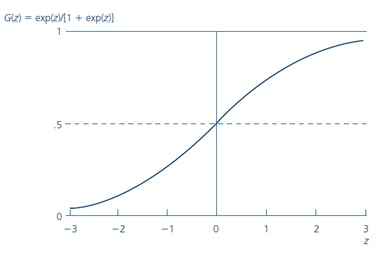
\includegraphics[height=5.5cm]{ima11}
% \end{center}
% 
% Anexo2: Resultados de la aplicación del Modelo Probit
% \begin{center}
% 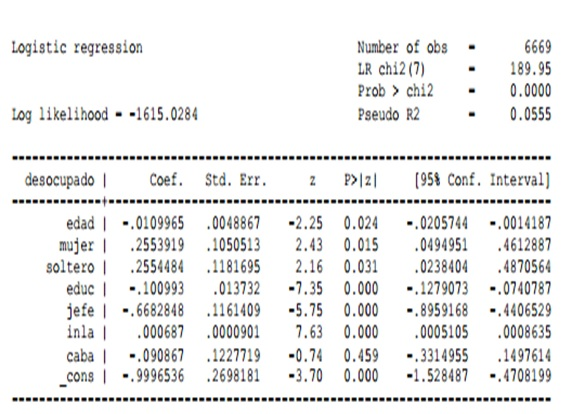
\includegraphics[height=6.5cm]{kat1}
% \end{center}
% 
% Anexo3: Resultados de la estimación con el Modelo Logit
% \begin{center}
% 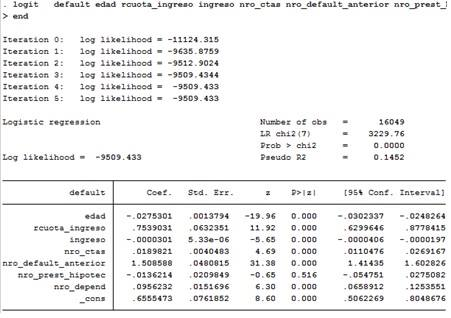
\includegraphics[height=8.5cm]{picture11}
% \end{center}
% 
% Anexo4: Resultados del Test de Wald
% \begin{center}
% 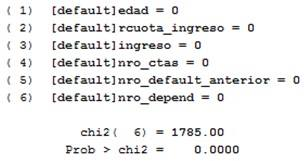
\includegraphics[height=4cm]{picture8}
% \end{center}
% 
% Anexo5: Resultados de la segunda estimación con el Modelo Logit \begin{center}
% 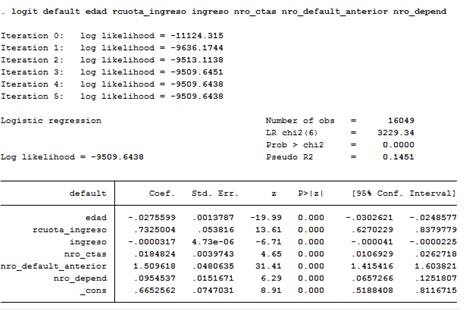
\includegraphics[height=8.5cm]{picture7}
% \end{center}
% 
% \newpage
% Anexo6: Resultados de la estimación con el Modelo Probit
% \begin{center}
% 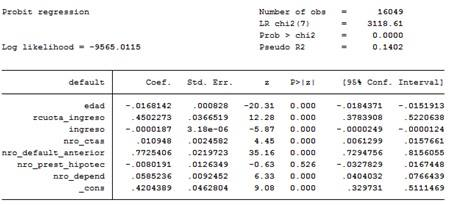
\includegraphics[height=6.5cm]{picture1}
% \end{center}
% 
% Anexo7: Resultados de la segunda estimación con el Modelo Probit
% \begin{center}
% 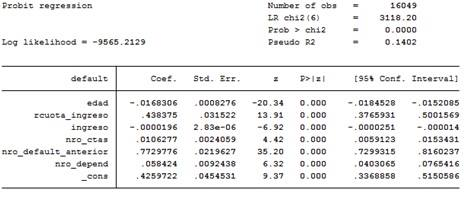
\includegraphics[height=6.5cm]{picture10}
% \end{center}
% 
% Anexo8: Potencia de la predicción con el Modelo Logit
% \begin{center}
% 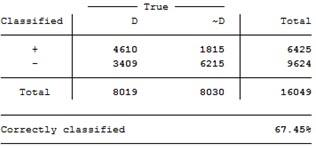
\includegraphics[height=5.5cm]{picture4}
% \end{center}
% 
% \newpage
% Anexo9: Potencia de la predicción con el Modelo Probit
% \begin{center}
% 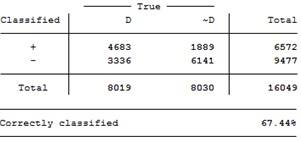
\includegraphics[height=5.5cm]{picture3}
% \end{center}
% 
% Anexo10: Representación gráfica de la Curva ROC
% \begin{center}
% 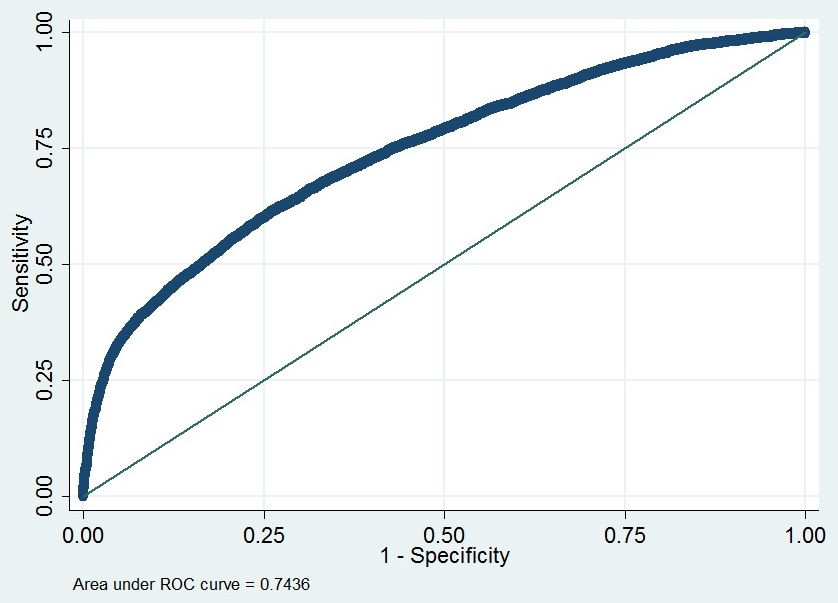
\includegraphics[height=7cm]{picture16}
% \end{center}
% 
% Anexo11: Valor esperado de la PD por categoría
% \begin{center}
% 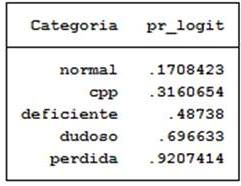
\includegraphics[height=5.5cm]{picture6}
% \end{center}
% 
% Anexo12: Pérdida esperada de la entidad financiera ABC por categoría
% \begin{center}
% 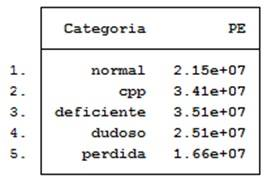
\includegraphics[height=5.5cm]{picture2}
% \end{center}
% 
% 
% %----------------
% \chapterimage{cc} % Chapter heading image
% 
% 
% %Anexos
% \chapter*{Conclusiones}
% \section{Analisis}\index{Conclusiones}
% \addcontentsline{toc}{chapter}{\textcolor{ocre}{Anexos}}
% 
% Anexo1: Representación gráfica de la función logística
% \begin{center}
% 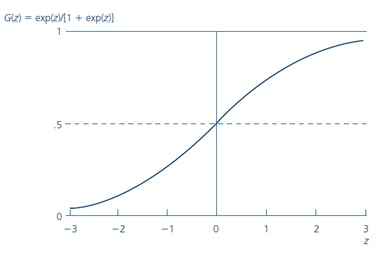
\includegraphics[height=5.5cm]{ima11}
% \end{center}
% 
% %----------------------------------------------------------------------------------------
% %	BIBLIOGRAPHY
% %----------------------------------------------------------------------------------------
% \chapterimage{KL} % Chapter heading image
% \chapter{Bibliografía}
% \addcontentsline{toc}{chapter}{\textcolor{ocre}{Bibliografía}}
% \section*{Books}
% \addcontentsline{toc}{section}{Books}
% \printbibliography[heading=bibempty,type=book]
% \section*{Articles}
% \addcontentsline{toc}{section}{Articles}
% \printbibliography[heading=bibempty,type=book]
% 
% \begin{itemize}
% 	\item GREENE, W.H. (2003) “Econometric Analysis”5ª edición. Prentice Hall N.J. Capítulo 21
% \\\\
%     \item WOOLDRIDGE, J.M. (2010) “Introducción a la Econometría: Un Enfoque Moderno". 4ª edición. Cengage Learning. Capítulo 17
% 
% \end{itemize}
% 
% 
% %----------------------------------------------------------------------------------------
% %	INDEX
% %----------------------------------------------------------------------------------------
% 
% \cleardoublepage
% \phantomsection
% \setlength{\columnsep}{0.75cm}
% \addcontentsline{toc}{chapter}{\textcolor{ocre}{Índice Alfabético}}
% \printindex
% 
% %----------------------------------------------------------------------------------------

\end{document}
